\documentclass{article}
\usepackage{iclr2026_conference,times}
\usepackage[T1]{fontenc}
\usepackage[utf8]{inputenc}
\usepackage{amsmath,amssymb,amsthm,booktabs,graphicx,array,multirow}
\usepackage{xcolor}
\usepackage{hyperref}
\usepackage{url}
\usepackage{etoolbox}
\setcitestyle{citesep={,},yysep={,}}
\makeatletter
\patchcmd{\@maketitle}{Paper under double-blind review}{Paper under anonymous review}{}{}
\makeatother
% Avoid automatic word splitting in the manuscript.
\hyphenpenalty=10000
\exhyphenpenalty=10000
\emergencystretch=2em
\hypersetup{colorlinks=true,linkcolor=blue!55!black,citecolor=blue!55!black,urlcolor=blue!55!black,
 pdftitle={AutoMF: Automated Ensembles for Multifidelity Field Prediction},pdfauthor={Anonymous authors}}
\newcommand{\method}{\textsc{AutoMF}}
\newcommand{\R}{\mathbb{R}}
\newcommand{\E}{\mathbb{E}}
\newcommand{\calD}{\mathcal{D}}
\newcommand{\simplex}{\Delta_M}
\newcommand{\norm}[1]{\left\lVert#1\right\rVert}
\newtheorem{proposition}{Proposition}
\newcounter{algorithm}
\title{AutoMF: Automated Ensembles\\for Multifidelity Field Prediction}
\author{Anonymous authors}
% Anonymous ICLR review layout. The manuscript has not been submitted.
\begin{document}
\maketitle
\begin{abstract}
Learning to predict physical fields requires fine simulation data that can be
expensive to obtain. Multifidelity learning combines inexpensive coarse solutions
with fine data to improve generalization to new parameter inputs, but the most
effective way to use these fidelities varies across problems. We present
\method{}, an automated ensemble workflow for multifidelity field prediction.
We construct its library by adapting neural operators, convolutional networks,
and reduced basis models into nine parameter to field surrogates. For each dataset, five additional input and
fine solution pairs, reserved from surrogate training, guide model selection
and ensemble weighting. The workflow either selects an individual model,
weights models according to their individual errors, or jointly fits weights
to minimize the combined prediction error. Each model receives one weight that
remains fixed across the field and across new inputs, allowing prediction
without an additional coarse simulation. We assemble a benchmark of 22 datasets
spanning seven classes of partial differential equations (PDEs) and climate
emulation, combining our simulations with imported data to compare individual
models, additional baselines, and ensembles. Different models lead on different datasets, motivating their
combination. Compared with selecting the lowest error individual model,
the fitted ensemble improves accuracy on 16
datasets and reduces geometric mean relative $L^2$ error by 11.6\% when averaged
across PDE classes and 7.5\% when averaged across all datasets.
\end{abstract}

\begin{figure}[h!]
\centering

\includegraphics[width=\linewidth]{figures/graphical_abstract.pdf}
\caption{\textbf{An ERA5 example from training data to field prediction.}
The input $x$ comprises 12 emissions variables and the target $y$ is a fine ERA5
temperature field \citep{hersbach2020,niu2024}. Five reserved fine examples
determine inverse error weights $w_m$ for nine model fields $f_m(x)$, whose weighted average is
$\widehat y(x)$. Each weight applies across the whole field. The training pair
shares one input, while predictions use a separate reserved input.}
\label{fig:overview}
\end{figure}

\section{Introduction}
Scientific design requires solution fields for many choices of physical
parameters. Changing a boundary condition or diffusivity changes the temperature
throughout a domain. A surrogate model learns this map without repeating fine
simulations. Multifidelity learning adds cheaper coarse solutions
\citep{kennedy2000,howard2023,niu2024}, leaving a practical choice: which model
should use them? Transfer learning, joint training, and coarse field correction
use different fidelity relationships, and their accuracy can change as those
relationships weaken \citep{faza2026}.

We train a surrogate library and use additional known fine solutions to fit
ensemble weights. \method{} compares three
rules: select the most accurate individual model, average models according to
their individual errors, or fit averaging weights to minimize the combined
error. New parameters
produce a fine field without another coarse solve (Figure~\ref{fig:overview}).
Each dataset has its own fitted ensemble, with one weight per model fixed across
inputs and grid points. Automation selects and combines models within prescribed
training recipes.

An ensemble increases surrogate computation while reusing expensive field data.
For climate modeling, the Regional Aerosol Model Intercomparison Project
(RAMIP) reports indicative costs of approximately 100{,}000 CPU core hours for
CESM2.1 and 400{,}000 for UKESM1 per coupled simulation spanning roughly
36 simulated years \citep[Appendix~A]{wilcox2023ramip}. Core hours measure total
processor usage. These figures describe RAMIP simulations, not the production
cost of our ERA5 archive. \citet[Section~6]{niu2024} similarly describe their
extra inference overhead as ``small compared with the actual simulators''.
When generating fields dominates the budget, additional surrogate computation
can therefore be reasonable. \method{} reuses available training fields across
candidates and the same reserved fine examples across selection and combination
rules.

This approach builds on engineering surrogate ensembles
\citep{goel2007,acar2009,viana2009}, automated model libraries
\citep{feurer2015,erickson2020}, and comparative studies of multifidelity field
surrogates \citep{brunel2025}. Our contribution has three connected parts.
First, we construct a library of nine field surrogates by adapting established
architectures to transfer, pooled supervision, coarse field correction, and
fine only prediction. A common parameter to field interface makes these
different uses of training data available for selection and combination.
Second, we assemble a benchmark of 22 datasets from our simulations and imported
data, documenting their fidelity definitions and comparing models on common
evaluation cases within each dataset. Third, \method{} connects this library
and benchmark through an automated ensemble workflow with an explicitly counted
budget of additional fine solutions. The underlying architectural components
and ensemble weighting principles are established.

We first compare individual library models with additional baselines, then
ask whether ensemble fitting improves on choosing one model. Error analysis,
fitting loss controls, and ERA5 climate emulation \citep{hersbach2020,niu2024}
examine when combining predictions helps. This separates library accuracy from
reliable selection. Historical results informed development, so these
comparisons remain retrospective.

\section{Background: from surrogate selection to field ensembles}
\label{sec:related}
Engineering studies already show why choosing one surrogate can be difficult
and why combining several can help. \citet{goel2007} weight surrogates using
error estimates, \citet{acar2009} and \citet{stromberg2021} optimize metamodel weights, and
\citet{viana2009} compare cross validation selection, weighted prediction, and
library subsets. For functional outputs, \citet{brunel2025} compare more than
a dozen multifidelity surrogates in a common framework. Their findings connect
model performance to fidelity correlation, training size, and residual
complexity. These studies establish both the ensemble principle and the need
for comparisons across problems. We extend this empirical line of work to a
surrogate library for fields and measure combination gains under small,
explicitly counted fitting budgets.

The weighting rules follow stacked generalization \citep{wolpert1992}, stacked
regression \citep{breiman1996}, and Super Learner \citep{superlearner2007}.
Greedy ensemble selection \citep{caruana2004}, auto sklearn
\citep{feurer2015,feurer2022}, and AutoGluon \citep{erickson2020} automate
selection from broader libraries. Related multifidelity workflows automate
other parts of the process: EL MFS combines low fidelity models inside
hierarchical fusion \citep{wang2024elmfs}, AQBMF screens low fidelity information
and surrogate candidates \citep{lee2026aqbmf}, and the MAESTRO preprint screens
families by leave one out validation \citep{kim2026maestro}. Our ensemble fitting
stage acts on completed target field predictions from different fidelity
strategies. We evaluate that stage and its library, without a direct comparison
against these complete engineering automation systems.

The library draws on Fourier neural operators (FNO) \citep{li2021fno}, DeepONet
\citep{lu2021}, wavelet neural operators (WNO) \citep{tripura2022wno}, and Transolver
\citep{wu2024transolver}. Multifidelity operator learning also includes
DeepONet \citep{howard2023}, MF WNO \citep{thakur2022mf}, and FNO for carbon
storage \citep{tang2023}. MFRNP uses decoded coarse outputs in residual prediction
\citep{niu2024}, while FIRE uses coarse predictive distributions
\citep{yu2026fire}. Appendix~\ref{app:adaptations} identifies the components we
adapt and the departures from their original formulations. HyperNOs addresses
automated operator training \citep{ghiotto2025}, and LANE SI combines sea ice
fields \citep{borisova2024}. PDEBench and The Well supply broader physical
benchmarks \citep{takamoto2022,ohana2024}. Our study starts from supplied training
data and fits ensemble weights, leaving simulation acquisition to approaches
such as active multi resolution learning \citep{li2024active}.

\section{AutoMF: model selection and ensemble fitting}
\label{sec:method}
\subsection{From parameter inputs to field predictions}
At fidelity $\ell$, the training data are
$\calD_\ell=\{(x_i^{(\ell)},y_i^{(\ell)})\}_{i=1}^{N_\ell}$: $N_\ell$ examples
indexed by $i$, each pairing $d$ simulation parameters $x_i^{(\ell)}\in\R^d$
with a field $y_i^{(\ell)}$ on grid $\Omega_\ell$. The index $\ell$ identifies
fidelity. Each surrogate model $f_m$ maps the parameter vector $x$
to a fine field on a common target grid. For models that incorporate a coarse
field, this field is obtained internally: either a trained low fidelity
surrogate model predicts it at $x$, or nearest neighbour retrieval selects the stored
coarse solution whose training parameters are closest to $x$ in standardized
parameter space. The coarse field then serves as a reference for a learned
correction. Thus, $f_m$ denotes the complete inference procedure, including any
coarse prediction, retrieval, and correction, and requires no additional
simulation at the query input.

We reserve $K$ additional fine examples for \emph{ensemble fitting} and a separate evaluation set.
We refer to the reserved input and fine field pairs as \emph{fitting examples}.
Both sets are excluded from low fidelity (LF) and high fidelity (HF) training
before normalization, basis construction, or model fitting. Input identities
establish correspondence between fidelities. Each dataset has its own trained
surrogate library and ensemble weights. Each rule determines its weights from
the fitting examples and saves them before scoring evaluation fields.
Appendix~\ref{app:splits} discusses split integrity and prior access to
historical evaluation results.

\subsection{Surrogate model library}
The surrogate library contains nine models, M1 to M9 in Table~\ref{tab:paperbaselines},
chosen to vary both the representation of a field and the way coarse data
enter learning. Transfer can reuse features across fidelities, joint supervision
shares information during training, and correction uses a coarse field as a
spatial reference. A fine only reduced basis model supplies an alternative
when coarse information is less useful. We adapt these strategies to the same
parameter input and target field interface, including the internal coarse
prediction or retrieval required by correctors. Three models first learn from coarse fields
and then finetune on fine fields, following multifidelity transfer learning
\citep{lyu2023}. FiLM FNO transfer combines Fourier mixing
\citep{li2021fno} with parameter conditioned featurewise linear modulation
(FiLM) \citep{perez2018}.
ConvNeXt transfer uses convolutional blocks in an encoder and decoder with skip
connections \citep{liu2022convnext}. Wavelet transfer uses a custom wavelet
representation inspired by WNO \citep{tripura2022wno}. Together they test coarse
initialization across different spatial representations. All pairs FNO instead
pools supervision across fidelity pairs before fine training. It takes
parameters and two fidelity labels as inputs. Poseidon motivates pair enumeration
\citep{herde2024}, while our FNO \citep{li2021fno} uses neither its temporal
operator nor a supplied source field.

Four models use coarse predictions or retrieved fields to guide a correction.
Distribution FNO predicts a residual from coarse ensemble summaries, adapting
FIRE's distribution conditioning idea \citep{yu2026fire}. Retrieved field
DeepONet uses a branch and trunk representation \citep{lu2021,lu2022mf} to
correct a neighboring coarse training field. The slice attention and ConvNeXt
correctors refine a predicted coarse field through six updates, using modified
Transolver inspired attention \citep{wu2024transolver} and convolutional blocks
\citep{liu2022convnext}, respectively. Their coarse inputs are assembled out of
fold with four ensemble members per case. Finally, POD GP predicts coefficients
in a proper orthogonal decomposition (POD) basis using Gaussian processes (GP)
\citep{higdon2008}. It tests whether a compact field representation can be
learned directly from fine solutions. Our adaptations specify how parameters
condition each model, how fidelities supervise it, and how coarse references
are constructed. Appendix~\ref{app:adaptations} explains for each model
the source components, our changes, and the inclusion rationale. Architecture and training cost
both vary across the library, so rankings cannot be attributed to one design
choice alone.

\subsection{Fitting one weight per model}
The ensemble averages the model predictions,
\begin{equation}
 \widehat y_w(x)=\sum_{m=1}^M w_m f_m(x),\qquad
 w\in\simplex=\{w\in\R^M:w_m\geq0,\ \mathbf{1}^\top w=1\}.
 \label{eq:mixture}
\end{equation}
Here $M=9$ counts models, $w_m$ weights model $m$, and $\widehat y_w$ is the
combined field. The simplex $\Delta_M$ contains nonnegative weights summing to
one. The vector $\mathbf{1}$ contains ones and $\top$ denotes transpose.
Weights stay fixed across inputs and grid points. For fitting pair $(x_i,y_i)$,
define $\langle a,b\rangle_Q=a^\top Qb$, $\norm a_Q=\sqrt{a^\top Qa}$, and
$s_i=\max(\norm{y_i}_Q,10^{-8})$. Fields are vectors of grid values, $Q=I$ is
the identity matrix, and the floor prevents division by zero. We compute
\begin{equation}
 e_{im}=\frac{f_m(x_i)-y_i}{s_i},\qquad
 [G_i]_{mn}=\langle e_{im},e_{in}\rangle_Q,\qquad
 \widehat C=\frac{1}{K}\sum_{i=1}^K G_i.
 \label{eq:gram}
\end{equation}
Here $e_{im}$ is model $m$'s relative error field on example $i$, $G_i$ records
error products between models $m$ and $n$, and $\widehat C$ averages these over
$K$ fields. Diagonal entries measure individual squared error. Other entries
measure error alignment, retaining information needed to score a mixture.

\noindent\textbf{Selected model.} This rule gives weight one to model $m^*$
with the lowest mean relative $L^2$ error on the fitting examples,
$m^*=\arg\min_m K^{-1}\sum_i\sqrt{[G_i]_{mm}}$.

\noindent\textbf{Inverse error mixture.} This rule gives more weight to individually
accurate models:
\begin{equation}
 w_m^{\rm inv}=\frac{1/\max(\widehat C_{mm},\tau)}
 {\sum_j 1/\max(\widehat C_{jj},\tau)},\qquad \tau=10^{-30}.
\label{eq:inverse}
\end{equation}
Here $w_m^{\rm inv}$ is the normalized inverse error weight, $j$ runs over all
models, and $\tau$ prevents division by zero. The weights sum to one.

\noindent\textbf{Fitted mixture.} This rule chooses the weights together by minimizing
the error of their combined prediction:
\begin{equation}
 \widehat w^{\rm full}\in\arg\min_{w\in\simplex}w^\top\widehat Cw.
 \label{eq:stack}
\end{equation}
Here $\widehat w^{\rm full}$ minimizes the mean squared relative error
$w^\top\widehat Cw$ on the fitting examples. This is convex stacking
\citep{wolpert1992,breiman1996}, allowing a less accurate model to offset another's errors.
Both mixture rules use squared normalized errors, whereas model selection and
reporting use mean relative $L^2$. The objectives can have different optima.
We test the consequence of this choice in Section~\ref{sec:results} and derive
the distinction in Appendix~\ref{app:geometry}. Numerical details appear in
Appendix~\ref{app:numerics}.

Ensemble fitting estimates only nine weights, with eight free values because
they sum to one. The surrogate models remain fixed, and each fitting field
supplies spatial error products that summarize individual accuracy and error
alignment. Once these products are computed, the optimization uses a
$9\times9$ matrix regardless of the number of grid points. This small fitting
problem makes limited additional fine data a practical option. Spatial values
within a field remain dependent, however, so field resolution does not count
as additional independent fitting examples or guarantee generalization from
five fields. Appendix~\ref{app:algorithm} gives the pseudocode.

\section{Evaluating the surrogate library and ensemble}
\label{sec:experiments}
\subsection{Datasets and comparison coverage}
We assemble a benchmark of 22 datasets spanning elliptic equations, diffusion,
convection, shocks, porous flow, reaction diffusion, waves, and ERA5 climate
emulation \citep{hersbach2020,niu2024}. Figure~\ref{fig:datasets} shows one fine
field from each dataset, illustrating the range of field structures and grid
resolutions. The collection combines our simulations with
imported parameter and field data, using different grids or data sources as
fidelities. Euler, Burgers, and Shallow water use the published PyClaw finite
volume framework \citep{ketcheson2012pyclaw}. Their problem designs include
Euler quadrant configurations motivated by The Well \citep{ohana2024} and a
radial dam break adapted from PDEBench \citep{takamoto2022}. Custom solvers
are supported by targeted analytical and numerical checks, including a
Barenblatt solution test for Porous medium and mesh refinement for Allen Cahn
(Appendix~\ref{app:generatorchecks}). Several datasets describe the same governing equation, so the
roster represents 22 prediction tasks rather than 22 independent physical
families (Appendix~\ref{app:roster}).

We evaluate all nine library models and their ensembles on all 22 datasets.
Models are trained using the training examples available for each dataset,
with additional fine examples reserved for ensemble fitting. Reported
comparisons use the same evaluation cases within each dataset and fitting
partition. Each final surrogate model uses a single seed. Baseline settings, model
specific training schedules, fitting and validation allocations, and comparison
coverage are detailed in Appendices~\ref{app:protocol}
and~\ref{app:matchedbaselines}.

\begin{figure}[t]
\centering
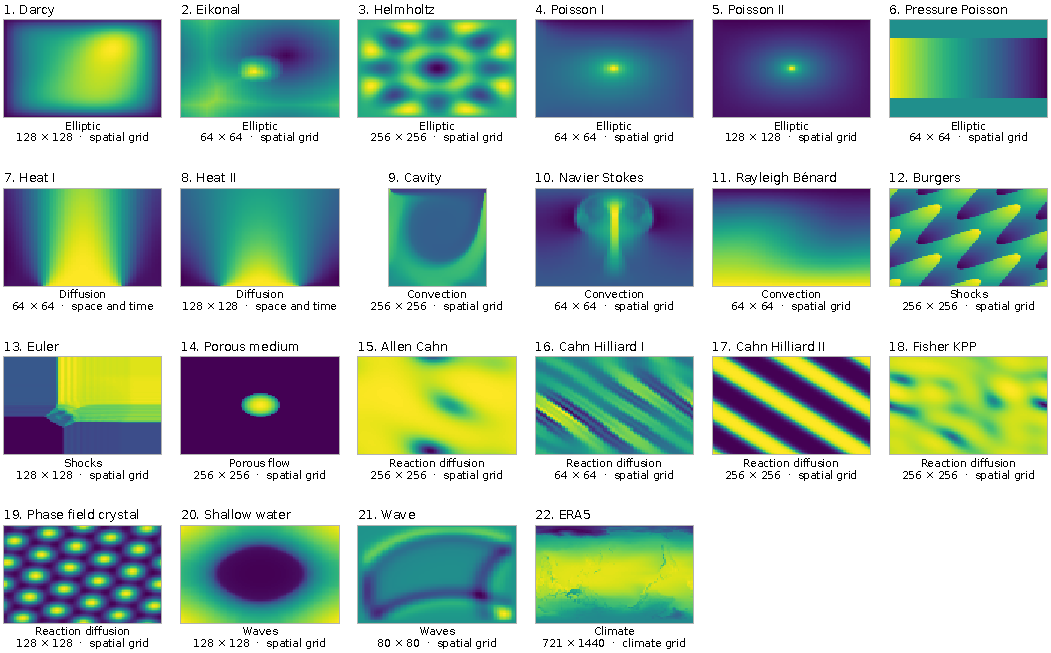
\includegraphics[width=\linewidth]{figures/dataset_gallery.pdf}
\caption{\textbf{The 22 datasets span different field structures.} Panels are
grouped by class and show one fine training field per dataset with its native grid size. Heat fields span space
and time, and the cavity shows vorticity. ERA5 predictions use a
$128\times256$ working grid. Display conventions are described in
Appendix~\ref{app:gallery}. Imported data: Poisson II, Heat II, and Navier Stokes
\citep{niu2024}, and ERA5 \citep{hersbach2020,niu2024}.}
\label{fig:datasets}
\end{figure}

\subsection{Ensemble fitting budgets and evaluation}
For each PDE dataset, we keep the trained models fixed and ask how many
additional fine solutions are needed to choose their mixture. We compare
$K\in\{5,10,20\}$ fitting examples, each consisting of an input and its known
fine field. These examples are separate from surrogate training and evaluation.
Every rule receives the same $K$ examples for selecting an individual model
or fitting mixture weights. We then measure prediction error on
separate evaluation cases shared by all methods. We repeat this comparison
using three partitions of fitting and evaluation cases without retraining
the models. This measures sensitivity to the choice of fitting examples.
Split construction and case counts are given in Appendix~\ref{app:splits}.

We report mean relative $L^2$ error, averaging over cases and then partitions.
To compare proportional changes across datasets, we aggregate error ratios
geometrically. Dataset aggregation gives each dataset equal weight. PDE class
aggregation first averages within each class and then gives the classes equal
weight:
\begin{equation}
 \rho_{a/b}=\exp\!\left[\frac1{|\mathcal C|}\sum_{c\in\mathcal C}
 \frac1{|\mathcal D_c|}\sum_{d\in\mathcal D_c}\log\frac{\bar E_{d,a}}{\bar E_{d,b}}\right].
 \label{eq:aggregate}
\end{equation}
Here $a,b$ denote methods, $\bar E_{d,a}$ is method $a$'s partition averaged error
on dataset $d$, $\mathcal C$ is the set of PDE classes, and $\mathcal D_c$ contains
class $c$'s datasets. Vertical bars count set members. The ratio $\rho_{a/b}$ gives
each class equal weight, with values below one favoring $a$. The two summaries answer
different questions: a dataset in a singleton class has six times the weight
of one elliptic dataset under class aggregation. Wins and losses require more
than a 1\% relative change. This is a descriptive threshold, not a significance
test. Tables express errors as percentages and improvements as relative changes.

\section{Results: from a surrogate library to a fitted ensemble}
\label{sec:results}
\subsection{Different models lead on different datasets}
The library contains strong individual models, but their relative accuracy
depends on the prediction task. Seven of its nine members achieve the lowest
error on at least one PDE dataset. Wavelet transfer leads on Darcy, POD GP on
the Poisson variants, and distribution FNO on the heat variants, while the
ConvNeXt corrector leads on Cavity and Euler. The four additional reaction
diffusion tasks each favor a different library member. This variation motivates keeping
several ways of using coarse information available: choosing one architecture
for the entire collection would discard models that are useful on particular
problems. Table~\ref{tab:allexperts} shows these differences directly, placing
each individual model beside the ensemble rules and the strongest additional
baseline for each dataset.

The best library member outperforms the best available additional baseline on
15 of the 21 PDE datasets. Here the best model in each collection is identified
after evaluation, so this comparison measures the accuracy available within
the library. The fitted mixture also achieves lower aggregate error than the
best additional baseline, while individual baselines remain preferable on
some datasets (Appendix~\ref{app:headlines}). The next question is whether the
reserved fitting examples can turn this available accuracy into a useful
prediction rule. Table~\ref{tab:paperbaselines} summarizes the aggregate
comparisons and Elo ranking, with individual baseline errors in
Appendix~\ref{app:matchedbaselines}.

\begin{table}[t]
\centering\fontsize{7}{8.5}\selectfont\setlength{\tabcolsep}{2.3pt}
\caption{\textbf{Comparing the library, its combinations, and additional baselines.}
All columns report mean relative $L^2$ error in percent on the same evaluation
cases. The best additional baseline is identified by its B label, and M1 to M9
are defined in Table~\ref{tab:paperbaselines}. The selected model uses one member,
the inverse error mixture weights individual errors, and the fitted mixture
optimizes their combination. All three use five fitting examples. Bold marks the lowest unrounded evaluation error.
Daggers mark exclusions in the separate sensitivity analysis
(Appendix~\ref{app:subsets}). Section~\ref{sec:experiments} specifies coverage.
Imported data: Poisson II, Heat II, and Navier Stokes \citep{niu2024}, and ERA5
\citep{hersbach2020,niu2024}.}
\label{tab:allexperts}
\resizebox{\linewidth}{!}{\begin{tabular}{lr|rrrrrrrrr|rrr}
\toprule
Dataset & Best baseline & M1 & M2 & M3 & M4 & M5 & M6 & M7 & M8 & M9 & \shortstack[r]{Selected\\model} & \shortstack[r]{Inverse\\error\\mixture} & \shortstack[r]{Fitted\\mixture} \\
\midrule
Darcy & 3.37 (B1) & 3.07 & 3.44 & 2.78 & 4.98 & \textbf{2.32} & 31.7 & 3.37 & 3.41 & 3.41 & 2.52 & 2.55 & 2.33 \\
Eikonal & 2.21 (B8) & 2.42 & 2.15 & 1.81 & 4.79 & 2.59 & 7.37 & 3.63 & 3.74 & 2.95 & 1.81 & 1.76 & \textbf{1.76} \\
Helmholtz & 4.12 (B9) & \textbf{3.3} & 3.48 & 4.79 & 10.9 & 5.04 & 29.1 & 7.1 & 10.9 & 10.8 & 6.25 & 6.89 & 6.55 \\
Poisson I & \textbf{0.00531} (B2) & 0.0413 & 0.0387 & 0.0427 & 0.0611 & 0.0955 & 9.92 & 0.00684 & 0.128 & 0.0838 & 0.00684 & 0.008 & 0.00788 \\
Poisson II$^{\dagger}$ & 0.0128 (B1) & 0.256 & 0.536 & 0.2 & 25.5 & 0.881 & 26.6 & \textbf{0.0121} & 0.921 & 0.798 & \textbf{0.0121} & 0.0125 & 0.0129 \\
Pressure Poisson$^{\dagger}$ & 0.0639 (B9) & 0.0599 & 0.0695 & 0.0918 & 0.0871 & \textbf{0.0498} & 0.285 & 0.0922 & 0.309 & 0.145 & 0.0734 & 0.0769 & 0.0802 \\
Heat I & 0.0206 (B10) & 0.0164 & 0.0125 & 0.0105 & 0.00915 & 0.0268 & 2.28 & 0.327 & 0.0494 & 0.0149 & 0.00972 & \textbf{0.00593} & 0.0062 \\
Heat II & 0.0201 (B10) & 0.0139 & 0.00878 & 0.00859 & 0.00662 & 0.0173 & 1.58 & 0.312 & 0.0268 & 0.0121 & 0.00662 & 0.00437 & \textbf{0.00435} \\
Cavity & \textbf{0.0419} (B5) & 98.5 & 0.29 & 98.5 & 0.681 & 3.6 & 70.1 & 0.409 & 2.06 & 0.164 & 0.164 & 0.142 & 0.142 \\
Navier Stokes & 1.52 (B10) & 1.55 & 1.69 & 1.57 & 1.58 & 2.33 & 4.41 & 2.79 & 2.62 & 1.95 & 1.61 & 1.52 & \textbf{1.5} \\
Rayleigh Bénard & 0.011 (B10) & 0.0112 & 0.00915 & 0.00715 & 0.00301 & 0.0137 & 0.0999 & 0.295 & 0.0529 & 0.0195 & 0.00301 & 0.00286 & \textbf{0.00269} \\
Burgers & 0.562 (B9) & 0.547 & 0.533 & 100 & 0.507 & 1.28 & 4.88 & 2.5 & 1.69 & 0.545 & 0.516 & 0.513 & \textbf{0.502} \\
Euler & \textbf{5.54} (B2) & 6.2 & 6.08 & 6.72 & 6.3 & 7.43 & 8.13 & 6.15 & 6 & 5.88 & 6.09 & 5.64 & 5.73 \\
Porous medium & 0.0718 (B9) & 0.0448 & 0.0325 & 0.0596 & 0.0654 & 0.126 & 2.75 & 0.909 & 0.681 & 0.0497 & 0.0325 & \textbf{0.0262} & 0.0263 \\
Allen Cahn & 41.2 (B5) & 53 & 52.7 & 42.1 & 45.4 & 41.3 & 102 & 55.5 & 41.4 & 38.8 & 39.4 & 37.9 & \textbf{34.6} \\
Cahn Hilliard I$^{\dagger}$ & 13.3 (B10) & 12.9 & 12.5 & 12.2 & 11.7 & 36.3 & 81.6 & 30.3 & 41.1 & 12.5 & 12.2 & 11.3 & \textbf{10.7} \\
Cahn Hilliard II & 49.8 (B5) & \textbf{46.9} & 48.3 & 51.9 & 50.8 & 60.8 & 99.8 & 64.8 & 55.9 & 47.8 & 52.2 & 47.2 & 49.3 \\
Fisher KPP & 3.24 (B9) & 3.21 & 3.22 & 2.36 & 2.98 & 3.83 & 6.49 & 6.86 & 2.86 & 2.84 & 2.36 & 2.53 & \textbf{2.3} \\
Phase field crystal & 83.5 (B11) & 89.6 & 89.5 & 111 & 83.3 & 202 & 120 & 83.5 & 85.3 & 85.7 & 83.5 & 83.8 & \textbf{83.3} \\
Shallow water & 0.403 (B10) & 0.428 & 0.367 & 0.362 & 0.876 & 0.446 & 1.38 & 1.09 & 1.29 & 0.502 & 0.367 & \textbf{0.357} & 0.389 \\
Wave & \textbf{3.3} (B3) & 6.36 & 6.31 & 4.75 & 11.1 & 5.04 & 64.2 & 24.9 & 8.35 & 11.3 & 4.84 & 4.39 & 4.27 \\
\midrule ERA5 & \textbf{5} (B1) & 14.2 & 17.7 & 20.4 & 12.2 & 9.75 & 9.54 & 6.74 & 20.4 & 8.24 & 6.74 & 5.81 & 6.49 \\
\bottomrule
\end{tabular}
}
\end{table}

\begin{table}[t]
\centering\fontsize{7.5}{9}\selectfont\setlength{\tabcolsep}{3pt}
\caption{\textbf{Model sources and performance, ranked by Elo.}
For each dataset, ratios divide a method's mean evaluation error by the
Selected model's error before geometric averaging. The Selected model is the
member of M1 to M9 with the lowest mean relative $L^2$ error on the five fitting
examples. \textbf{PDE class ratio} averages within each class
and then equally across the seven PDE classes (21 datasets).
\textbf{Dataset ratio} weights all 22 datasets equally, including ERA5.
A ratio of 1 matches selection, 0.90 means 10\% lower aggregate error, and
1.10 means 10\% higher aggregate error. Elo compares each pair of methods on all
22 datasets, with higher ratings better (Appendix~\ref{app:elo}).
M1 to M9 form the library, and B1 to B11
are additional baselines.
Citations identify components or ideas, with adaptations in
Appendix~\ref{app:adaptations}. Individual errors appear in
Table~\ref{tab:allexperts} and Appendix~\ref{app:matchedbaselines}.
Training costs and fine data budgets differ.}
\label{tab:paperbaselines}
\resizebox{\linewidth}{!}{\begin{tabular}{llrrr}
\toprule
Model / rule & Component or idea source & PDE class ratio & Dataset ratio & Elo \\
\midrule
Fitted mixture & \citep{breiman1996} & 0.884 & 0.925 & 1988 \\
Inverse error mixture & \citep{goel2007} & 0.888 & 0.932 & 1951 \\
Selected model & Fitting set selection & 1.000 & 1.000 & 1851 \\
M2 All pairs FNO & \citep{li2021fno,herde2024} & 1.333 & 1.541 & 1688 \\
M1 FiLM FNO transfer & \citep{li2021fno,perez2018} & 1.940 & 2.035 & 1642 \\
M9 ConvNeXt corrector & \citep{liu2022convnext} & 1.695 & 1.867 & 1634 \\
M3 ConvNeXt transfer & \citep{liu2022convnext} & 2.607 & 2.445 & 1619 \\
M4 Distribution FNO & \citep{yu2026fire} & 1.795 & 2.155 & 1592 \\
B10 FNO transfer II & \citep{lyu2023} & 1.794 & 1.850 & 1590 \\
B9 FNO transfer I & \citep{lyu2023} & 1.794 & 1.848 & 1578 \\
M5 Wavelet transfer & \citep{tripura2022wno} & 2.459 & 2.400 & 1528 \\
B5 Latent MF network & \citep{li2022dmfal} & 3.794 & 2.772 & 1497 \\
M7 POD GP & \citep{higdon2008} & 5.492 & 3.108 & 1450 \\
B1 Autoregressive POD GP & \citep{kennedy2000} & 5.854 & 3.362 & 1449 \\
M8 Slice attention corrector & \citep{wu2024transolver} & 4.189 & 3.549 & 1439 \\
B2 Nonlinear POD GP & \citep{perdikaris2017} & 5.871 & 3.626 & 1424 \\
B3 Composite MF MLP & \citep{meng2020} & 4.174 & 3.974 & 1387 \\
B8 Fidelity basis FNO & \citep{li2022ifc} & 8.979 & 6.217 & 1364 \\
B4 Composite MF DeepONet & \citep{howard2023} & 8.001 & 5.803 & 1337 \\
B11 Affine POD GP & \citep{zhang2018} & 17.624 & 11.236 & 1218 \\
B6 Nonlinear decoder transfer & \citep{seidman2022} & 9.927 & 8.252 & 1197 \\
M6 Retrieved field DeepONet & \citep{lu2022mf} & 20.847 & 14.890 & 1057 \\
B7 MFRNP adapter & \citep{niu2024} & 49.969 & 24.194 & 1020 \\
\bottomrule
\end{tabular}
}
\end{table}


\subsection{Combining predictions often improves accuracy}
Using the same five fitting examples, the fitted mixture improves on the
Selected model on 16 of 22 datasets. It reduces geometric mean relative
$L^2$ error by 11.6\% across PDE classes and 7.5\% across all datasets.
Both rules make their decisions before observing the evaluation fields, so
this comparison tests how effectively they use the available fine solutions.
The advantage over a best individual model identified retrospectively from
evaluation answers is much smaller and depends on aggregation
(Appendix~\ref{app:headlines}). The practical benefit is therefore lower error
when model choice must be made before the next fine field is known, with
failures as well as improvements visible in Table~\ref{tab:allexperts}.
Figure~\ref{fig:fieldcomparison} provides one field example.

\begin{figure}[t]
\centering
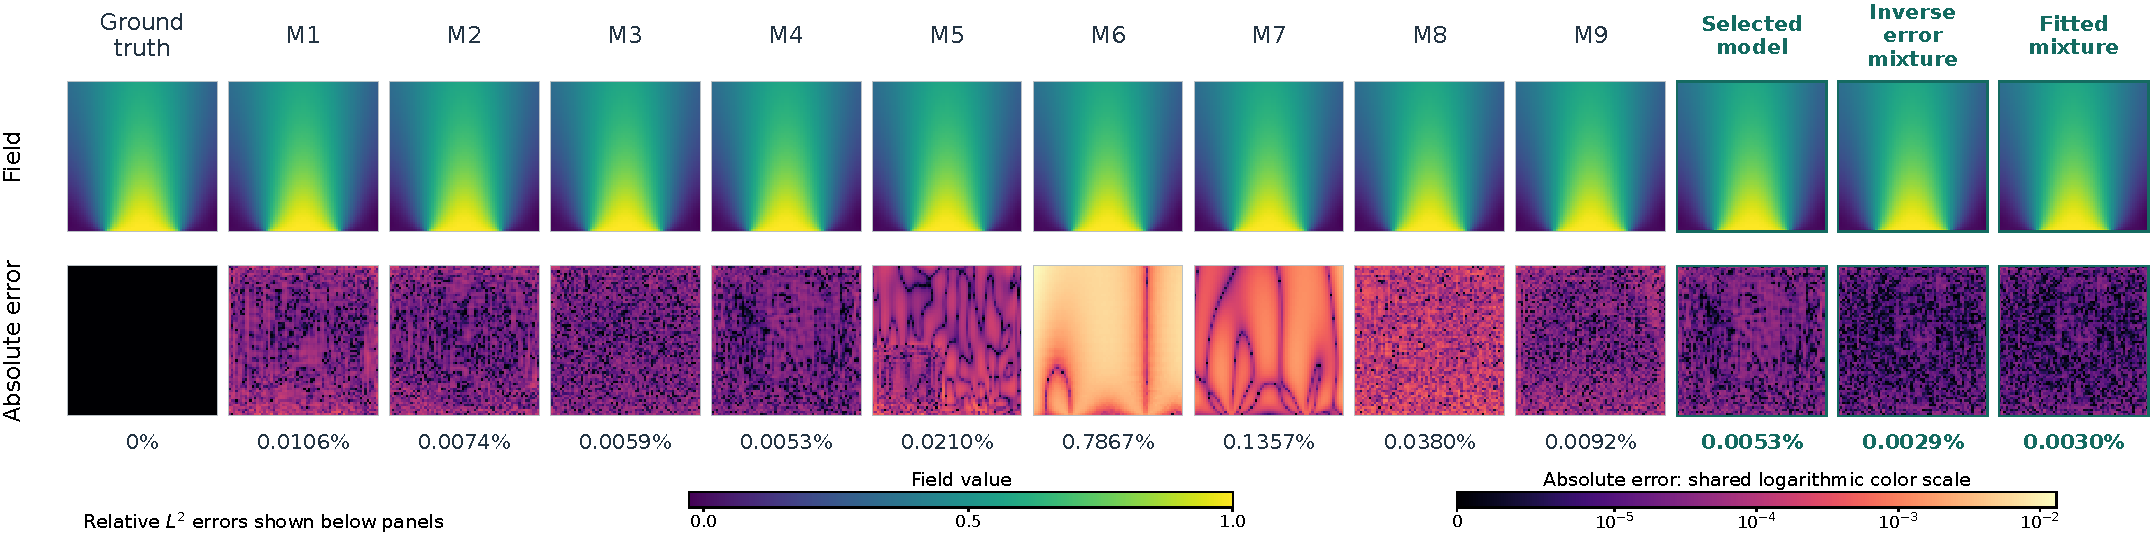
\includegraphics[width=\linewidth]{figures/field_comparison_heat.pdf}
\caption{\textbf{Combining models reduces field error on a Heat I example.}
Top: ground truth, nine model predictions, and the selected model, inverse error
mixture, and fitted mixture.
Bottom: absolute error on a shared logarithmic color scale, with relative $L^2$
error below each panel. Fields share a linear color scale and a $64\times64$ space and time grid.
The three rules use five fitting examples. The selected model is M4 here.
The case is the first evaluation input of the first
partition. The fitted mixture lowers error by 44.4\% relative to the best
individual model.}
\label{fig:fieldcomparison}
\end{figure}

\subsection{Simple weighting captures most of the benefit}
The inverse error mixture nearly matches the fitted mixture in aggregate
accuracy, and the two occupy the highest Elo positions in
Table~\ref{tab:paperbaselines}. Uniform averaging performs poorly
(Table~\ref{tab:main}), indicating that which models receive weight
matters. Yet individual model errors already provide a useful guide to those
weights, with only a small additional gain from joint fitting. The error
analysis supports complementary predictions as a source of improvement
(Appendix~\ref{app:geometry}). Both weighting rules can benefit from that
complementarity, even though the inverse error mixture does not explicitly
estimate interactions between model errors.

\subsection{Sensitivity to fitting and evaluation choices}
The advantage over model selection persists when more fine examples are
available for fitting. Across the 21 PDE datasets, increasing the allowance
from five to twenty examples raises the fitted mixture's reduction in
class aggregated geometric mean relative $L^2$ error from 11.6\% to 13.1\%
(Appendix~\ref{app:budgets}). Both methods receive the same allowance at each
budget, and the surrogate models remain fixed. The modest increase supports
using a small fitting set in these experiments, while leaving the amount
needed for a new problem to be assessed.

Two diagnostics use the same 17 dataset subset to examine dependence on the
evaluation design. Repeating the comparisons on fixed dataset subsets preserves the gain over the Selected
model, while superiority to the best individual model remains sensitive to
the comparison (Appendix~\ref{app:subsets}). We also minimize the reported mean
relative $L^2$ error directly, keeping the trained models and fitting examples
fixed. This gives a modest improvement over fitting squared relative error
(Table~\ref{tab:losscontrol}), identifying the fitting objective as a useful
design choice. This retrospective control is reported separately from the
three main rules.

\section{Analysis: why averaging can help}
\label{sec:analysis}
Averaging can improve predictions when spatial errors partly offset. For a
fixed library, classical ensemble analysis writes the expected squared relative
error as
\begin{equation}
 R(w)=\E[w^\top G(x,y)w]=w^\top Cw,\qquad C=\E[G(x,y)].
 \label{eq:riskmain}
\end{equation}
Here $G(x,y)$ is the error product matrix for a new input and target pair,
$\E$ averages over such pairs, $C$ is its population mean, and $R(w)$ is the
mixture's expected squared relative error. Its diagonal measures individual
error and its other entries retain alignment and shared bias
\citep{breiman1996,krogh1994}. The inverse error mixture can exploit complementary
predictions even though it uses only individual accuracy to choose weights.

This identity does not guarantee useful weights from a small fitting set,
and the bound in Appendix~\ref{app:proof} does not certify accuracy from five fields.
The reported metric $L(w)=\E[\sqrt{w^\top Gw}]$ averages unsquared relative error
and can favor different weights from $R$ even with unlimited fitting data.
Appendix~\ref{app:geometry} gives a counterexample and a direct fitting control.

\section{Application to climate field emulation}
\label{sec:climate}
ERA5 asks whether the workflow remains useful beyond the simulation datasets.
The task maps 12 emissions related inputs to temperature fields, combining
MFRNP's climate assembly \citep{niu2024} with ERA5 reanalysis
\citep{hersbach2020}, in the climate emulation setting motivated by ClimateBench
\citep{climatebench2022}. It contains 55 fine training inputs, ten fitting
inputs, and seven evaluation inputs. Reserved inputs are excluded from all
training fidelities. All nine models predict on a $128\times256$ working grid.


POD GP is the most accurate of the nine library models on ERA5, with a mean
relative $L^2$ error of 6.7369\%. With five fitting examples, the inverse error
mixture reduces this error to 5.8146\%, a 13.69\% relative improvement. The
fitted mixture reaches 6.4877\%, improving by 3.70\%. Both mixtures therefore
improve on the best individual model in the library. Table~\ref{tab:allexperts}
shows the individual models and mixtures alongside the strongest additional
baseline, with all baseline results in Appendix~\ref{app:matchedbaselines}.

\section{Discussion and limitations}
\label{sec:discussion}
The findings connect the diversity of the surrogate library to a practical
model choice procedure. Different representations and uses of coarse data
provide accurate predictions on different problems. Reserved fine examples
then guide how much each model contributes before the next field is known.
Mixtures often improve on selecting one model, while inverse error weighting
shows that much of this gain is accessible through individual error estimates.
For an application with expensive simulations, additional surrogate computation
can therefore be a useful way to exploit the available fields. Once the library
is trained, comparing and fitting the three rules reuses its predictions without
retraining the models.

These results do not isolate a benefit specific to multifidelity data. The library includes
a fine only model, many datasets have equally sized coarse and fine training
tables, and validation allocations vary. Establishing data efficiency requires a
fine only library and alternative uses of fitting labels under equal total
label and computation budgets, counting every candidate and shared coarse
ensemble. Whether the additional surrogate computation is worthwhile depends
on simulation cost, the number of prediction queries, and the required accuracy.
Net cost savings and comparison with complete engineering automation systems
remain open.

\section{Conclusion}
The strongest surrogate for multifidelity field prediction changes across
problems. \method{} combines an adapted library of nine neural and reduced
basis models with an ensemble fitting workflow. Reserved fine solutions
determine which models to select or combine, and new inputs require no
additional coarse simulation. The assembled benchmark compares these choices
across field structures and fidelity relationships.

Across 22 datasets, the fitted mixture improves on selecting one model on 16
datasets using five reserved fine examples. Inverse error weighting captures most of this benefit.
ERA5 extends the comparison beyond PDE simulations. These findings support ensemble
fitting when uncertain model choice and expensive field data justify additional
surrogate computation.

\label{main:end}

\clearpage
\bibliographystyle{iclr2026_conference}
\phantomsection\label{references:start}
\bibliography{references}
\label{references:end}
\clearpage
\appendix
\phantomsection\label{appendices:start}
% Appendix roadmap follows the experimental workflow.
\section{Datasets and evaluation protocol}
\label{app:roster}
\subsection{Dataset definitions}
Table~\ref{tab:roster} describes the 22 prediction tasks. Here $d$ counts input
parameters, $N_H$ counts HF training rows, and $N_{L,\min}$ is the smallest LF
table, not the sum over fidelities. Query inputs are excluded from every
training fidelity and are subsequently partitioned into fitting and evaluation
sets. These counts describe available data, rather than identical exposure
under every training recipe. The seven PDE classes contain six elliptic,
two diffusion, three convection, two shock, one porous flow, five reaction
diffusion, and two wave datasets. ERA5 supplies the climate case and enters
dataset aggregation, but not PDE class aggregation.

\begin{table}[h!]
\centering\footnotesize\setlength{\tabcolsep}{3pt}
\caption{\textbf{Dataset definitions and available training data.} Query counts
include fitting pools and evaluation cases. Work grids are used for prediction
and scoring. Citations identify imported data, while uncited entries use our
simulation code.}
\label{tab:roster}\resizebox{\linewidth}{!}{\begin{tabular}{lrrrrrll}
\toprule
Dataset & $d$ & Levels & $N_{L,\min}$ & $N_H$ & Query & Work grid & Class \\
\midrule
Darcy & 16 & 3 & 400 & 400 & 100 & $128\times128$ & Elliptic \\
Eikonal & 3 & 2 & 400 & 400 & 100 & $64\times64$ & Elliptic \\
Helmholtz & 2 & 3 & 400 & 400 & 100 & $256\times256$ & Elliptic \\
Poisson I & 5 & 3 & 400 & 400 & 100 & $64\times64$ & Elliptic \\
Poisson II \citep{niu2024} & 5 & 5 & 64 & 64 & 512 & $128\times128$ & Elliptic \\
Pressure Poisson & 2 & 4 & 400 & 400 & 100 & $64\times64$ & Elliptic \\
Heat I & 3 & 3 & 400 & 400 & 100 & $64\times64$ & Diffusion \\
Heat II \citep{niu2024} & 3 & 5 & 1024 & 1024 & 512 & $128\times128$ & Diffusion \\
Cavity & 1 & 4 & 400 & 400 & 100 & $256\times256$ & Convection \\
Navier Stokes \citep{niu2024} & 2 & 2 & 256 & 256 & 256 & $64\times64$ & Convection \\
Rayleigh Bénard & 1 & 2 & 400 & 400 & 100 & $64\times64$ & Convection \\
Burgers & 2 & 3 & 400 & 400 & 100 & $256\times256$ & Shocks \\
Euler & 7 & 3 & 400 & 400 & 100 & $128\times128$ & Shocks \\
Porous medium & 2 & 3 & 400 & 400 & 100 & $256\times256$ & Porous flow \\
Allen Cahn & 19 & 3 & 400 & 400 & 78 & $256\times256$ & Reaction diffusion \\
Cahn Hilliard I & 2 & 2 & 400 & 400 & 100 & $64\times64$ & Reaction diffusion \\
Cahn Hilliard II & 19 & 3 & 400 & 400 & 100 & $256\times256$ & Reaction diffusion \\
Fisher KPP & 50 & 3 & 400 & 400 & 100 & $256\times256$ & Reaction diffusion \\
Phase field crystal & 18 & 3 & 400 & 400 & 100 & $128\times128$ & Reaction diffusion \\
Shallow water & 2 & 3 & 400 & 400 & 100 & $128\times128$ & Waves \\
Wave & 3 & 2 & 400 & 400 & 100 & $80\times80$ & Waves \\
ERA5 \citep{hersbach2020,niu2024} & 12 & 9 & 313 & 55 & 17 & $128\times256$ & Climate \\
\bottomrule
\end{tabular}
}
\end{table}

Poisson II, Heat II, and Navier Stokes use data released with MFRNP
\citep{niu2024}. ERA5 combines its climate model sources with reanalysis targets
\citep{hersbach2020,niu2024}. Other entries were simulated for this collection.
Pressure Poisson adapts an analytic construction motivated by \citet{partin2022},
Euler a quadrant setup motivated by The Well \citep{ohana2024}, and Shallow
water a radial dam break recipe motivated by PDEBench \citep{takamoto2022}.
These recipe influences do not make the independently simulated entries copies
of those benchmarks. Euler, Burgers, and Shallow water call PyClaw
\citep{ketcheson2012pyclaw}, using first order Godunov methods at coarse
fidelities and SharpClaw WENO reconstruction at the fine fidelity. Our dam
break varies both the inner water height and radius on a unit square, with
independent solves at each grid. Phase field crystal implements the conserved
dynamics of \citet{elder2004}. Roman numerals distinguish tasks with the same equation.
Poisson I and II have related parameterizations, while Cahn Hilliard I and II
have 2 and 19 input parameters. Cahn Hilliard II, Allen Cahn, and Fisher KPP use
$64\times64$, $128\times128$, and $256\times256$ fidelity grids. Phase field
crystal uses $32\times32$, $64\times64$, and $128\times128$ grids. Their input
dimensions are 19, 19, 50, and 18, respectively. Heat fields span space and
time, and Helmholtz predicts amplitude normalized fields.

\phantomsection
\label{app:generatorchecks}
\noindent\textbf{Numerical checks and their scope.}
Verification scripts test the custom implementations against analytical
solutions, conservation laws, and refined numerical solutions. In a one
dimensional Barenblatt test \citep{vazquez2007}, the Porous medium solver's
relative $L^2$ error falls from $8.1\times10^{-4}$ at 128 points to
$2.6\times10^{-5}$ at 512 points. An Allen Cahn mesh check reduces error
from $4.9\times10^{-5}$ at 64 points to $2.3\times10^{-6}$ at 256 points
against a 512 point reference. The archived checks also test mass conservation
for Cahn Hilliard II and Phase field crystal, and the Helmholtz discrete
equation residual. These are controlled checks of selected solver components,
including one dimensional tests for solvers used in two dimensions. They do
not certify every sampled parameter or the accuracy of every stored field.
The companion package records the scripts, measured errors, and scope of
each check. Published software and recipe references establish provenance,
while the implementation checks are our own.

Related archives can share physical simulations, so the 22 tasks are not
independent samples of PDE families. Three entries have additional limitations:
Poisson II has inherited numerical defects, Cahn Hilliard I omits realization
information from its parameters, and Pressure Poisson uses synthetic coarse
fields. Appendix~\ref{app:subsets} checks sensitivity to these entries without
certifying the other solvers.

\subsection{Training, fitting, and evaluation cases}
\label{app:splits}
Reserved fitting and evaluation inputs are excluded from LF and HF training
before normalization, basis construction, or model fitting. Within each PDE
partition, input hashes separate fitting from evaluation and define nested
budgets $K\in\{5,10,20\}$. Every rule uses the same fitting allowance, including
any selection or tuning. Models remain fixed across three partitions, which
measure sensitivity to case assignment rather than variation across training
seeds. Some cases change roles between partitions. Across the 21 PDE datasets,
3,058 query rows produce 1,842 evaluation appearances corresponding to 1,505
distinct dataset and row pairs. Shared simulations across related datasets can
further reduce physical independence. Historical evaluation results influenced
development and reporting scope, making these comparisons retrospective.

Allen Cahn, Cahn Hilliard II, Fisher KPP, and Phase field crystal each supply
400 training inputs per fidelity. Their query pools contain 78, 100, 100, and
100 inputs. Each partition reserves 16 evaluation cases for Allen Cahn and
20 for each of the other three datasets. ERA5 has 55 HF training inputs,
ten fitting pool inputs, and seven evaluation inputs, with a smallest retained
LF table of 313 rows. The additional Heat I inputs in
Appendix~\ref{app:additionalheat} form a separate supplementary evaluation.
The subset and loss diagnostics cover the original 17 PDE tasks, while the
primary comparison covers all 22 datasets.

Predictions share target grids, scaling, and input identities within each
comparison. Source hashes, saved target identities, or checkpoint evaluation
verify correspondence. Saved weights are fixed before evaluation answers are
scored, and replay checks reproduce individual errors, mixture errors, and
aggregate denominators. ERA5 answer files are separated from model training,
and changing evaluation answers leaves fitted weights unchanged in the
collector check. These checks verify the implemented separation without
reconstructing all prior researcher access. Error matrices use float64 and
the same stored model predictions are reused within each experiment.
Precision and checkpoint provenance records remain in the companion package.

\subsection{How the fields are displayed}
\label{app:gallery}
Figure~\ref{fig:datasets} shows row zero of each HF training table, chosen
independently of prediction error. Its grids are native array grids, while
the inventory gives the working grids used for scoring. Heat axes span space
and time. The cavity target is vorticity, with the top lid moving right and
array rows increasing upward. Its display uses a symmetric logarithmic scale,
linear within $[-1,1]$ and bounded by $[-400,400]$, so wall values do not hide
the interior structure. No values are clipped or modified. Enlarged panels,
numerical display scales, extraction metadata, and source hashes for all
22 datasets are included in the companion package.

Figure~\ref{fig:fieldcomparison} illustrates Heat I, selected after inspecting
dataset results. It uses the first evaluation case of the first partition,
not the case with the greatest improvement, and reuses the saved five example
fits. All predicted fields share a linear color scale. Absolute errors share
a logarithmic scale that is linear between zero and $10^{-5}$. Scores use
the complete $64\times64$ fields without smoothing. The selected model is M4,
so its column repeats that model. Figure~\ref{fig:overview}'s ERA5 display
uses a smoothed coarse thumbnail and interpolates the predicted working grid
to the native fine grid for illustration, without changing scored fields.

\clearpage
\section{Model adaptations and training}
\label{app:protocol}
The library varies both the representation of a field and how coarse data
enter learning. We first identify the retained published components and our
adaptations, then give the training settings. The additional baseline
descriptions use the same distinction between a source idea and a complete
published method.

\subsection{Model sources, adaptations, and rationale}
\label{app:adaptations}
Each library member combines a field representation with a training and inference
procedure. We describe M1 to M9 individually below, identifying the published
components retained, the changes made for parameter to field prediction, and
the reason for including each model. Several members combine ideas from more
than one paper. The resulting library is an integration of adapted models,
not nine independent reproductions or nine newly proposed architectures.
All accept parameters alone at deployment. Appendix~\ref{app:experts} gives
their training budgets and data use. The rationales below motivate the library's
composition, while the experiments assess its predictions. They do not isolate
the effect of every architectural change.

\paragraph{M1: FiLM FNO transfer.}
The starting components are FNO's learned Fourier mixing \citep{li2021fno},
FiLM's featurewise affine conditioning \citep{perez2018}, and the LF pretraining
followed by HF finetuning strategy of \citet{lyu2023}. We retain spectral
convolutions with local residual paths and adapt the input interface to a
simulation parameter vector. The spatial input contains coordinates only.
At each block, a parameter network generates a scale and shift applied after
group normalization, so the parameters influence features throughout the
network. Related parameter conditioning for PDE emulation is studied by
\citet{shokar2025}. Our model differs from our parameter concatenation FNO references, which
supply parameters as constant spatial channels at the input. The same weights
are first trained on LF fields and then finetuned on HF fields. This combination
tests whether repeated parameter conditioning and a coarse initialization
provide an effective way to generate globally coupled fields.

\paragraph{M2: All pairs FNO.}
M2 retains M1's FNO and FiLM components \citep{li2021fno,perez2018} and adapts
the idea of pair enumeration from Poseidon \citep{herde2024}. Poseidon uses
pairs of states for temporal operator learning. Here the pairs index source
and target fidelities. We append their normalized labels to the parameter
vector, pool the corresponding target fields on a common working grid, and
train one conditional FNO before HF finetuning. The source label specifies a
training pair, but no source field enters the network. Poseidon's architecture,
pretrained weights, and temporal operator are not used. For ERA5, exact input
joins retain each target field with its own parameters. The purpose is to let
one model share information across fidelity tasks before specializing to the
fine field. Pair enumeration also repeats targets and changes optimization
cost, so its effect cannot be attributed to fidelity conditioning alone.

\paragraph{M3: ConvNeXt transfer.}
ConvNeXt supplies the depthwise spatial convolution, channel expansion, and
residual block structure \citep{liu2022convnext}. We place these blocks in an
U shaped encoder and decoder with skip connections \citep{ronneberger2015} and
a dense field output, adapting the image classification backbone to field
generation. The model starts from
coordinates and replaces the usual block normalization with group normalization
and FiLM conditioning on the simulation parameters \citep{perez2018}. Three
downsampling stages and a bottleneck process the field at several resolutions,
with corresponding decoder stages restoring the target grid. LF pretraining
and HF finetuning follow the transfer principle of \citet{lyu2023}. The
rationale is to provide local spatial processing alongside M1's Fourier mixing,
while retaining the same type of parameter conditioning and transfer schedule.

\paragraph{M4: Distribution FNO.}
FIRE conditions a fine correction on summaries of a coarse predictive
distribution using tabular foundation models and in context inference
\citep{yu2026fire}. M4 retains the distribution conditioning idea and replaces
those models with FNOs trained on spatial fields \citep{li2021fno}. Five LF
members predict a coarse field at the query parameters. Their pointwise mean,
standard deviation, and 10th, 50th, and 90th percentiles become spatial input
channels for a residual FNO, together with coordinates and broadcast parameters.
The residual is added to the coarse mean to predict the fine field. Both stages
are trained by gradient optimization, so this implementation does not retain
FIRE's inference without model retraining. The ensemble summaries are features
of prediction variability, not a guarantee of accurate uncertainty estimates. The
rationale is to expose coarse disagreement as well as the mean to the
correction model. This recipe has no out of fold construction and is distinct
from the coarse ensembles used by M8 and M9.

\paragraph{M5: Wavelet transfer.}
WNO motivates learning in wavelet coordinates \citep{tripura2022wno}. We
replace M1's Fourier mixing with a custom single level db4 wavelet transform,
while retaining its coordinate input, FiLM conditioning \citep{perez2018},
local residual paths, and LF to HF transfer schedule \citep{lyu2023}. Within
each wavelet subband, learned weights mix channels at coefficient positions
inside a capped leading block. Other positions pass through unchanged before
the inverse transform. These indices describe positions within a subband,
not a Fourier frequency cutoff. The implementation also handles rectangular
grids, odd grid sizes, and one dimensional grids. It is a custom wavelet
representation rather than an exact reproduction of the published WNO.
Its inclusion tests whether spatially localized wavelet features provide useful
predictions alongside the spectral and convolutional transfer models.

\paragraph{M6: Retrieved field DeepONet.}
DeepONet supplies the branch and trunk representation \citep{lu2021}, while
the multifidelity use of a coarse prediction as a reference is motivated by
\citet{lu2022mf}. We use a Cartesian product DeepONet whose branch receives
the parameters concatenated with a stored LF training field and whose trunk
receives target grid coordinates. A nearest neighbour search in standardized
parameter space selects that field. The network learns a residual relative to
its interpolated version, which is then added back to form the fine prediction.
Retrieval is the deployment adaptation: a new query requires parameters only
and no new coarse solve. The rationale is to exploit a nearby physical field
without first learning a separate coarse surrogate. If an exact LF match exists
at a training input, retrieval supplies that match, whereas an unseen query
uses a neighboring input. This difference in reference quality remains a
limitation. The implemented residual model is also distinct from the composite
multifidelity architecture of \citet{howard2023}.

\paragraph{M7: POD GP.}
Basis emulation represents a large field through a small set of coefficients
\citep{higdon2008}. M7 retains this principle, constructing a POD basis by
singular value decomposition of centered HF training fields. A Gaussian process
maps parameters to each retained coefficient, and the predicted coefficients
are projected back through the basis and added to the training mean field.
Our implementation uses an RBF kernel with automatic relevance determination
and shares covariance hyperparameters across coefficient outputs. It does not
implement the full Bayesian hierarchy of the cited model. M7 is deliberately
fine only: no coarse field enters basis construction, fitting, or inference.
It supplies a compact alternative when the field varies mainly in a few
directions or when learning a coarse correction is less effective than learning
the fine coefficients directly.

\paragraph{M8: Slice attention corrector.}
Transolver motivates grouping spatial cells into learned slice tokens
\citep{wu2024transolver}. We retain pooled spatial summaries but change the
attention operation. Original Transolver normalizes each cell's assignments
across slices, applies attention between slice tokens, and maps back using
the assignments. Our pooling weights instead normalize across cells, and
cell queries attend directly to the pooled slice tokens. The model receives
the current field, coordinates with sinusoidal features, and FiLM conditioning
on the parameters \citep{perez2018}. A coarse surrogate ensemble supplies its
initial state, with out of fold predictions for training cases. A head
initialized to zero predicts additive corrections through six damped updates
with shared weights. Training penalizes spatial squared error and Fourier
magnitude discrepancy at each update, plus a nonzero update when started at
the target field. This encourages an equilibrium without guaranteeing
contraction. The adaptation tests whether pooled global interactions can
refine a predicted coarse field using parameters alone at deployment. Its
attention and iterative recipe differ from the published Transolver.

\paragraph{M9: ConvNeXt corrector.}
M9 retains ConvNeXt's spatial and channel mixing blocks \citep{liu2022convnext}
and adapts them to the same correction task as M8. It uses a custom U shaped
encoder and decoder with skip connections \citep{ronneberger2015}, three
downsampling stages and a bottleneck,
and FiLM parameter conditioning \citep{perez2018}. Unlike M3, which generates
a field from coordinates and parameters after transfer training, M9 receives
the current coarse estimate as a spatial input and outputs an additive update.
Its head is initialized to zero, making the initial refinement the identity.
The coarse ensemble construction, six damped updates, shared weights, and
spatial, spectral, and target state penalties follow the M8 recipe. The rationale
is to offer local processing at several resolutions as an alternative to pooled
attention when correcting the same kind of coarse prediction. This is a
ConvNeXt based iterative corrector, not the original classification model.

The additional baseline adaptations below use the same distinction between a
source idea and a complete published method. In particular, B1, B5, and B8 omit
central probabilistic components of co kriging, DMFAL, and IFC. Their scores
describe the implemented references, not faithful reproductions of those
complete methods. Common evaluation cases make the scores comparable while
leaving architecture and resource effects coupled.

\paragraph{B1, B2, and B11: classical multifidelity field references.}
B1 applies an autoregressive discrepancy idea \citep{kennedy2000} to POD GP field
models. It fits one scalar coupling coefficient in field space, constructs a
separate POD GP for residuals, and combines posterior means at deployment.
This is a plug in approximation rather than joint probabilistic co kriging.
B2 introduces nonlinear dependence on LF coefficients \citep{perdikaris2017}.
Its HF coefficient kernel combines input dependent coupling, an LF coefficient
kernel, and a discrepancy kernel. It shares covariance hyperparameters across
HF outputs and propagates marginal LF uncertainty through Monte Carlo samples.
B11 is a cheaper affine alternative inspired by multifidelity surrogate work
\citep{zhang2018}. One slope and one intercept are fitted jointly over HF training cases and
pixels, using observed LF fields when paired and emulated LF fields otherwise.
They are then applied to the LF POD GP prediction.
It does not fit an affine mapping separately for each mode. Paired training rows
can use observed LF fields, whereas deployment uses predicted LF fields.

\paragraph{B3, B4, and B5: neural fusion references.}
B3 uses the composite correlation idea of \citet{meng2020}. A tanh MLP maps
parameters and coordinates to an LF value. This stage is frozen before linear
and nonlinear HF networks are trained on the original inputs and LF prediction,
with weight decay on the nonlinear branch. B4 follows the composite DeepONet
idea \citep{howard2023}, predicting fixed coarse sensors with an LF DeepONet and
feeding parameters plus sensors to linear and nonlinear HF DeepONets. The LF
stage is frozen and the HF branches are trained jointly in a subsequent stage. B5 takes hierarchical
latent transfer as inspiration from DMFAL \citep{li2022dmfal}. It uses two encoders
and linear field decoders, with the second encoder receiving parameters and the
first latent vector. Joint LF and HF squared losses replace the probabilistic
objective. Both the variational last layer and active acquisition are omitted.
The name latent MF network reflects these substantial departures.

\paragraph{B6 and B7: alternative decoder and probabilistic models.}
B6 uses NOMAD's nonlinear decoding principle \citep{seidman2022}. A parameter MLP
produces a latent vector and a coordinate conditioned MLP decodes the field.
The model is implemented independently, with multifidelity learning supplied by
LF pretraining and HF finetuning. B7 directly imports MFRNP's upstream
\texttt{MultiFidelityModel} \citep{niu2024}. Its adapter changes data loading,
normalization, resizing, and training. A scalar mean and standard deviation from
the first fidelity normalize inputs, while outputs are scaled per fidelity.
The longest grid side is capped at 256, rectangular grids are supported, and
bilinear antialiased resizing replaces the upstream transform. Batch size is
limited by the smallest fidelity, with independent shuffling across fidelities.
When HF training has at most ten examples, all rows are retained and the context
fraction range changes from $[0.20,0.25]$ to $[0.40,0.60]$. Hidden width is 128,
latent width is 64, and there are three hidden layers. Adam uses learning rate
and epsilon of $10^{-3}$. HF likelihood receives weight two and LF likelihood
weight one. Latent summaries are saved from the final training batch. These are
protocol adaptations of an upstream model, rather than a reproduction of its
published experiment.

\paragraph{B8, B9, and B10: fidelity and transfer FNO references.}
B8 forms latent spatial channels with an FNO and mixes them with weights predicted
from $[\ell,\ell^2]$, the fidelity label and its square. These two features
condition the spatial basis weights on fidelity. It uses maximum absolute scaling
per fidelity, the nearest registered scaler for an intermediate fidelity, LF
warm up, and joint LF and HF finetuning. IFC motivates fidelity dependent
representation \citep{li2022ifc}, but its neural ODE and Gaussian process are
absent. The descriptive name fidelity basis FNO makes this distinction explicit.
B9 and B10 are two archived entries for parameter concatenation FNO transfer
\citep{lyu2023}. In the inspected release, their model files are byte identical
and their training scripts differ only in repository paths and reported
identifiers. The labels FNO transfer I and II distinguish saved result entries,
not independent baseline families. Their different saved scores remain
unexplained by the inspected source. Both are retained to make the archived
comparison auditable, but neither their number nor their score difference is
evidence for architectural diversity or a reproducible recipe difference.
For ERA5 and the four additional reaction diffusion datasets, the identical
recipe is fitted once and its predictions are explicitly reused for B10,
with no additional training cost.


\subsection{Training settings and data use}
\label{app:experts}
Table~\ref{tab:training} summarizes the library schedules. For M1, M2, M3,
and M5, AdamW uses batch size at most 16, weight decay $10^{-5}$, gradient
clipping at 1, and cosine decay to $10^{-6}$. Initial learning rates are
$10^{-3}$ for pretraining and $3\times10^{-4}$ for HF finetuning. The FNO
recipe uses width 64, four blocks, and up to 12 Fourier modes per direction,
subject to the grid cap. M4 also uses AdamW but starts both its LF members
and residual stage at $10^{-3}$. M6 uses width 256 and five affine layers of
that width in each branch and trunk specification, including the latent output,
with ReLU and Adam at $10^{-3}$. Detailed grid dependent definitions and fitted
hyperparameters are retained with the model implementations and metadata.

\begin{table}[h!]
\centering\small\setlength{\tabcolsep}{4pt}
\caption{\textbf{Library training schedules.} Epochs count passes through the
relevant training table. Optimizer steps and repeated refinement steps are
different quantities. Each final surrogate uses a single seed, with internal
coarse ensemble initializations prescribed by its recipe.}
\label{tab:training}
\begin{tabular}{p{.16\linewidth}p{.72\linewidth}}
\toprule
Models & Nominal training procedure \\
\midrule
M1, M3, M5 & 2,500 LF epochs, followed by 2,500 HF epochs. \\
M2 & 2,500 epochs over pooled fidelity pairs, followed by 1,250 HF epochs. \\
M4 & Five LF FNOs and one HF residual FNO, each trained for 2,500 epochs. \\
M6 & 125,000 Adam iterations on HF residual targets. \\
M7 & HF basis construction and coefficient GP fitting, without an epoch schedule. \\
M8, M9 & Coarse members request 30,000 optimizer steps, rounded to whole epochs.
Each corrector uses 6,000 optimizer steps and six refinement updates per prediction. \\
\bottomrule
\end{tabular}
\end{table}

M1, M3, M4, M5, and M6 use the lowest registered LF level. M2 pools pairs
across registered fidelities, M8 and M9 predict the finest registered LF
level, and M7 uses HF fields only. ERA5 consequently uses level one for the
transfer and retrieval recipes and level eight for the iterative correctors.
For M8 and M9, five LF folds each contain four members: plain and
heteroscedastic variants with two initializations each. Training cases receive
the mean from their held out fold. All query cases use the four members of
fixed fold zero. Corrector checkpoints are selected using training only
validation. M7's basis uses only HF base training fields. Its original estimator
state was not saved, so the common prediction export reconstructs that training
only fit and restores target scaling.

Baselines use the settings of the evaluated benchmark implementations, with
the adaptations above. Training, validation allocations, and computation vary
across recipes. For example, on Darcy, B3 to B5 use 360 fine rows for fitting
and 40 for internal validation, while B1, B2, and the transfer recipe fit
400 rows. Both allocations consume 400 fine labels before ensemble fitting.
The total fine data budget is $N_H^{\rm base}+K$, plus any additional HF labels
used for tuning, where $N_H^{\rm base}$ counts base training labels and $K$
counts ensemble fitting examples. Final evaluation labels are separate.
Computation includes every candidate and coarse member trained or evaluated,
even if its final weight is zero. Some timing records measure prediction
export rather than training, preventing a common training cost estimate.
Thus common evaluation cases do not establish equal resources or isolate a
multifidelity advantage over a matched fine only ensemble.


\clearpage
\section{Ensemble implementation}
\subsection{Numerical fitting}
\label{app:numerics}
The Selected model, Inverse error mixture, and Fitted mixture use the same
$K$ input and fine field pairs. Their definitions appear in
Section~\ref{sec:method}. For joint fitting, the empirical error matrix is
symmetrized and divided by
$\max(\operatorname{tr}(\widehat C)/M,10^{-30})$. Here the trace sums diagonal
errors and $M=9$ counts models. This positive scaling changes the objective
magnitude without changing the matrix condition number or the exact minimizer. SLSQP uses the analytic
gradient, bounds $0\leq w_m\leq1$, the unit sum constraint, tolerance
$10^{-12}$, and at most 300 iterations. Uniform weights and the lowest
diagonal singleton initialize separate solves. Finite solutions with unit sum
residual below $10^{-6}$ are clipped to nonnegative values and renormalized.
Feasible starting points remain candidates, and the lowest fitting objective
determines the retained weights. These checks establish numerical feasibility,
not generalization to new inputs.

Uniform averaging, used as a control in Table~\ref{tab:main}, assigns every
member weight $1/M$. Forming the error matrices costs $O(KM^2P)$ for $P$
values per field. Streaming predictions and keeping only these matrices
requires $O(KM^2)$ storage. These costs exclude surrogate training and inference.
The companion package preserves additional regularization, pair fitting, and
coarse input refresh experiments separately from the three main rules.

\subsection{From a trained surrogate library to a deployed ensemble}\label{app:algorithm}
\refstepcounter{algorithm}\label{alg:calibration}
\begin{center}
\fbox{\begin{minipage}{0.94\linewidth}\small
\textbf{Algorithm \thealgorithm: train models, fit the ensemble, and predict}\par
\textbf{Input:} LF/HF training tables, $K$ reserved fine cases, fixed model recipes,
and one prescribed rule: Selected model, Inverse error mixture, or Fitted mixture.\par
1. Check input identities and working grids within the dataset. Train the surrogate models
using training data only. Record unresolved units or simulation metadata.\par
2. Predict fields for the fitting inputs and compute $G_1,\ldots,G_K$.\par
3. Fit the prescribed rule on all $K$ cases using the definitions in Section~\ref{sec:method}.\par
4. Save preprocessing, model identities, and fitted weights.\par
\textbf{Predict:} combine model predictions at new parameters using Equation~\eqref{eq:mixture}.\par
\textbf{Evaluate:} score reserved fine answers only after saving these choices.
\end{minipage}}
\end{center}
The algorithm separates surrogate training from ensemble fitting. The bundled
program implements steps 2 to 4 and combines saved model predictions for new
inputs. Dataset adapters and base model training remain separate components.
The three rules use the same fitting and evaluation cases within each comparison.



\clearpage
\section{Complete results and fitting budgets}
\label{app:allresults}
\subsection{Individual models, baselines, and ensembles}
\label{app:matchedbaselines}
Table~\ref{tab:allexperts} reports all nine library members and the three
ensemble rules on every dataset. Table~\ref{tab:baseline_detail}
completes that comparison with individual
additional baseline errors. The latter include the parameter kNN and training
mean controls, which are outside the ranked B1 to B11 collection. Every ranked
method covers all 22 datasets. Errors average the same evaluation cases
within each partition, followed by the three partitions. ERA5 uses its separate
seven case evaluation set. Full precision values, per case errors, and replay
metadata are retained in the companion package.

\begin{table}[h!]
\centering\footnotesize
\caption{\textbf{Additional baseline errors across all 22 datasets.} Mean relative $L^2$
errors in percent. B1: Autoregressive POD GP. B2: Nonlinear POD GP.
B3: Composite MF MLP. B4: Composite MF DeepONet. B5: Latent MF network.
B6: Nonlinear decoder transfer. B7: MFRNP adapter. B8: Fidelity basis FNO.
B9 and B10: FNO transfer I and II. B11: Affine POD GP. B12: Parameter kNN.
B13: Training mean. Mixtures use five fitting examples and the same evaluation
cases. A dash marks an unavailable additional
control, not a missing ranked method. B9 and B10's implementation relationship
is described in Appendix~\ref{app:adaptations}. Imported data are from
MFRNP \citep{niu2024} and ERA5 reanalysis \citep{hersbach2020}.
Daggers identify the data quality exclusions in Appendix~\ref{app:subsets}.}
\label{tab:baseline_detail}
{\scriptsize\setlength{\tabcolsep}{2pt}
\renewcommand{\arraystretch}{1.15}
\resizebox{\linewidth}{!}{\begin{tabular}{lrrrrrrrrrrrrrrr}
\toprule
Dataset & B1 & B2 & B3 & B4 & B5 & B6 & B7 & B8 & B9 & B10 & B11 & B12 & B13 & \shortstack[r]{Inverse\\error\\mixture} & \shortstack[r]{Fitted\\mixture} \\
\midrule
Darcy & 3.37 & 3.66 & 4.03 & 6.66 & 5.91 & 5.2 & 12.4 & 5.55 & 5.27 & 5.28 & 3.6 & 21.5 & 38 & 2.55 & 2.33 \\
Eikonal & 3.49 & 2.99 & 3.12 & 3.35 & 3.38 & 2.65 & 3.62 & 2.21 & 2.33 & 2.34 & 4.88 & 5.51 & 31.8 & 1.76 & 1.76 \\
Helmholtz & 12.3 & 15.2 & 11.5 & 7.84 & 8.12 & 99.6 & 58.6 & 99.7 & 4.12 & 4.12 & 15.9 & 25.7 & 92 & 6.89 & 6.55 \\
Poisson I & 0.00731 & 0.00531 & 0.181 & 0.161 & 0.1 & 0.479 & 6.79 & 0.239 & 0.0804 & 0.0806 & 2.68 & 7.51 & 31.9 & 0.008 & 0.00788 \\
Poisson II$^{\dagger}$ & 0.0128 & 0.0306 & 0.635 & 1.72 & 0.849 & 3.93 & 11.7 & 82.1 & 0.355 & 0.357 & 2.01 & 12.3 & 38.5 & 0.0125 & 0.0129 \\
Pressure Poisson$^{\dagger}$ & 0.457 & 0.472 & 0.07 & 1.53 & 0.127 & 0.446 & 1.05 & 0.684 & 0.0639 & 0.0645 & 0.681 & 0.196 & 1.58 & 0.0769 & 0.0802 \\
Heat I & 0.326 & 0.327 & 0.0696 & 0.125 & 0.069 & 0.432 & 1.29 & 0.275 & 0.0207 & 0.0206 & 1.09 & 1.35 & 12.4 & 0.00593 & 0.0062 \\
Heat II & 0.312 & 0.312 & 0.111 & 0.183 & 0.0721 & 0.219 & 7.4 & 0.32 & 0.0202 & 0.0201 & 0.405 & 0.856 & 13.2 & 0.00437 & 0.00435 \\
Cavity & 0.307 & 0.409 & 23.9 & 4.99 & 0.0419 & 24.1 & 55.7 & 0.129 & 0.622 & 0.666 & 37.2 & 0.077 & 17.1 & 0.142 & 0.142 \\
Navier Stokes & 2.8 & 2.48 & 2.08 & 4.01 & 3.71 & 7.08 & 25.7 & 1.62 & 1.52 & 1.52 & 21.6 & 3.27 & 41.2 & 1.52 & 1.5 \\
Rayleigh Bénard & 0.283 & 0.295 & 0.0542 & 0.0588 & 0.0134 & 0.0613 & 4.5 & 0.78 & 0.0113 & 0.011 & 0.715 & 0.0575 & 9.1 & 0.00286 & 0.00269 \\
Burgers & 2.16 & 2.5 & 1.54 & 8.14 & 1.22 & 15.7 & 27.7 & 0.928 & 0.562 & 0.562 & 11.7 & 0.677 & 73.2 & 0.513 & 0.502 \\
Euler & 5.6 & 5.54 & 6.56 & 6.16 & 6.15 & 8.81 & 9.15 & 7 & 6.52 & 6.43 & 6.25 & 6.21 & 32.2 & 5.64 & 5.73 \\
Porous medium & 1.15 & 0.859 & 0.299 & 1.31 & 0.772 & 0.918 & 33.7 & 5.14 & 0.0718 & 0.0718 & 1.98 & 1.92 & 31.9 & 0.0262 & 0.0263 \\
Allen Cahn & 55.5 & 98.6 & 59.9 & 44.8 & 41.2 & 94.4 & 69 & 48.9 & 55.8 & 55.8 & 55.4 & 78.3 & 100 & 37.9 & 34.6 \\
Cahn Hilliard I$^{\dagger}$ & 29.7 & 27.8 & 53.5 & 48.7 & 27.6 & 61.1 & 74.7 & 14.2 & 13.4 & 13.3 & 72.3 & 20.6 & 99.9 & 11.3 & 10.7 \\
Cahn Hilliard II & 64.8 & 83.5 & 85 & 53.7 & 49.8 & 72.4 & 66.7 & 54.4 & 54 & 54 & 64.8 & 78 & 100 & 47.2 & 49.3 \\
Fisher KPP & 6.86 & 6.86 & 6.48 & 4.01 & 3.45 & 7.44 & 4.08 & 4.74 & 3.24 & 3.24 & 6.86 & 5.67 & 6.86 & 2.53 & 2.3 \\
Phase field crystal & 83.5 & 86.4 & 90.7 & 87.5 & 87.8 & 152 & 89.4 & 102 & 86.8 & 86.8 & 83.5 & 86.7 & 87.5 & 83.8 & 83.3 \\
Shallow water & 1.14 & 1.02 & 0.467 & 0.878 & 0.691 & 0.883 & 5.59 & 0.806 & 0.403 & 0.403 & 2.94 & 1.22 & 25.1 & 0.357 & 0.389 \\
Wave & 27.7 & 24.9 & 3.3 & 42.3 & 46.6 & 5.39 & 93.9 & 25.9 & 6.6 & 6.6 & 50.3 & 42.8 & 98.7 & 4.39 & 4.27 \\
\midrule ERA5 & 5 & 6.74 & 45 & 16.8 & 5.05 & 23.9 & 19.5 & 5.15 & 11.9 & 11.9 & 8.45 & 5.16 & 6.74 & 5.81 & 6.49 \\
\bottomrule
\end{tabular}
}}
\end{table}

\subsection{Library quality and the benefit of averaging}
\label{app:headlines}
Two comparisons separate the quality of the available library from the
benefit of combining it. The best library reference minimizes partition
averaged error over M1 to M9 separately for each dataset. The best additional
baseline minimizes the corresponding error over B1 to B11. Both use evaluation
answers retrospectively and are stronger references than the deployable
Selected model, which uses only fitting examples.
Table~\ref{tab:headlinecomparisons} reports these comparisons on the 21 PDE
datasets. Table~\ref{tab:paperbaselines} additionally includes ERA5 in its
dataset ratios and Elo ranking.

\begin{table}[h!]
\centering\small
\caption{\textbf{Library quality and mixture gains on the 21 PDE datasets.}
Ratios are geometric means. Wins and losses require a relative difference
greater than 1\%. Best library and best additional baseline refer to the
retrospective per dataset minima described above.}
\label{tab:headlinecomparisons}\begin{tabular}{lrrrr}
\toprule
Comparison & Class ratio & Dataset ratio & Wins & Losses \\
\midrule
Best library / best additional baseline & 0.766 & 0.834 & 15 & 5 \\
Fitted mixture / best library & 0.923 & 0.989 & 13 & 6 \\
Inverse error mixture / best library & 0.927 & 1.002 & 12 & 7 \\
Fitted mixture / best additional baseline & 0.706 & 0.825 & 13 & 7 \\
Fitted mixture / Selected model & 0.884 & 0.923 & 15 & 5 \\
\bottomrule
\end{tabular}

\end{table}

A still stronger control chooses a potentially different best model in each
partition using its evaluation answers. Against this reference, the fitted
mixture at $K=5$ has class ratio 0.933 and dataset ratio 1.006, with
13 improvements and 6 losses greater than 1\%. Thus its advantage over
retrospective model choice depends on both the reference and aggregation.

\subsection{Fitting budgets and uniform averaging}
\label{app:budgets}
Table~\ref{tab:main} compares the main rules with uniform averaging on the
21 PDE datasets. Table~\ref{tab:budgets} varies the fitting budget while keeping
the models and case partition protocol fixed. Each ratio compares methods that
receive the same number of fitting examples. These summaries measure sensitivity
to ensemble fitting, not independent training seed variation.

\begin{table}[h!]
\centering\small
\caption{\textbf{Weighting the same nine model library.} Ratios compare with
the Selected model at $K=5$ on 21 PDE datasets. Lower is better. Wins and losses
require changes larger than 1\%.}
\label{tab:main}\begin{tabular}{lrrrr}
\toprule
Method & Class balanced & Equal dataset & Wins & Losses \\
\midrule
Selected model & 1.000 & 1.000 & 0 & 0 \\
All pairs FNO & 1.333 & 1.502 & 3 & 15 \\
Uniform (all nine) & 5.919 & 4.944 & 2 & 19 \\
Inverse error mixture & 0.888 & 0.935 & 13 & 5 \\
Fitted mixture & 0.884 & 0.923 & 15 & 5 \\
\bottomrule
\end{tabular}

\end{table}

\begin{table}[h!]
\centering\small
\caption{\textbf{Increasing the fitting budget on the 21 PDE datasets.}
Class aggregated error ratios. The models remain fixed, and every comparison
uses the same allowance of $K$ additional fine fields.}
\label{tab:budgets}\begin{tabular}{rrrr}
\toprule
$K$ & \shortstack[r]{Inverse error mixture /\\Selected model} & \shortstack[r]{Fitted mixture /\\Selected model} & \shortstack[r]{Fitted mixture /\\Inverse error mixture} \\
\midrule
5 & 0.8876 & 0.8840 & 0.9958 \\
10 & 0.8921 & 0.8765 & 0.9826 \\
20 & 0.8900 & 0.8692 & 0.9766 \\
\bottomrule
\end{tabular}

\end{table}

\subsection{Elo ranking}
\label{app:elo}
Each pair of methods plays one comparison per dataset using its unrounded
partition averaged error. Lower error wins and an absolute difference below
$10^{-12}$ is a tie. The nine library members, eleven baseline entries, and
three rules all enter on the same 22 datasets. Ratings start at 1500. For
ratings $R_a,R_b$, the expected score and update are
\begin{equation}
 p_a=\frac{1}{1+10^{(R_b-R_a)/400}},\qquad
 R_a'=R_a+32(s_a-p_a),\qquad R_b'=R_b-32(s_a-p_a).
\end{equation}
Here $s_a$ is one for a win, zero for a loss, and one half for a tie.
Primes denote updated ratings. We reset ratings and independently shuffle
comparisons 500 times, then report the mean final rating. The code fixes the
random orders. Sorting uses unrounded ratings and display uses integers.
Datasets receive equal weight. Elo summarizes how often a method wins rather
than the magnitude of improvement, statistical significance, or training cost.

\clearpage
\section{Robustness checks and ERA5 details}
\label{app:reanalysis}
\subsection{Sensitivity to comparison scope}
\label{app:subsets}
The following diagnostics reuse the original 17 PDE tasks within the expanded
collection. They retain the trained models, predictions, and fitting cases.
The 14 task data quality subset excludes Poisson II, Cahn Hilliard I, and
Pressure Poisson for the properties described in Appendix~\ref{app:roster}.
A second subset removes Heat II and Burgers, the two tasks whose B8 case
correspondence was established through checkpoint evaluation. Their intersection
contains 12 tasks. Class aggregation normalizes over represented classes.
These retrospective sensitivity checks do not certify solver validity or
provide independent replication.

\begin{table}[h!]
\centering\small\setlength{\tabcolsep}{3pt}
\caption{\textbf{Sensitivity to dataset inclusion.} Each cell gives the PDE
class ratio followed by the dataset ratio. $N$ counts tasks. Library and
baseline refer to retrospective best models after averaging partitions.
Both mixtures use five fitting examples.}
\label{tab:reviewsensitivity}
\resizebox{\linewidth}{!}{\begin{tabular}{lrrrr}
\toprule
Scope & $N$ & Library / baseline & \shortstack[r]{Fitted mixture /\\Selected model} & \shortstack[r]{Inverse error mixture /\\Selected model} \\
\midrule
Diagnostic set & 17 & 0.764 / 0.820 & 0.876 / 0.918 & 0.882 / 0.924 \\
Data quality subset & 14 & 0.747 / 0.810 & 0.873 / 0.900 & 0.875 / 0.908 \\
Without Heat II and Burgers & 15 & 0.790 / 0.865 & 0.872 / 0.935 & 0.872 / 0.940 \\
Intersection & 12 & 0.776 / 0.865 & 0.869 / 0.918 & 0.865 / 0.926 \\
\bottomrule
\end{tabular}
}
\end{table}

Gains over the Selected model persist across these scopes. Superiority to the
best individual library member is less stable. On the 15 task subset, the
fitted mixture has class ratio 0.916 and dataset ratio 1.020 against that
reference, improving under one aggregation and worsening under the other.
The complete subset and budget tables remain in the companion package.

Source hashes also identify identical M8 and M9 prediction archives on Darcy.
These entries do not supply distinct prediction diversity on that dataset.
Their weights can be redistributed without changing a fitted combined field,
while inverse error weighting is affected by duplication because each copy
receives weight before normalization. Effective model count therefore measures
weight concentration over entries, not independent mechanisms. We retain the
evaluated library and disclose this property rather than interpreting those
weights as unique measures of model usefulness.

\subsection{ERA5 protocol and controls}
\label{app:climateprotocol}
\label{app:era5}
All nine library models use ERA5 training inputs disjoint from the ten fitting
pool and seven evaluation inputs \citep{hersbach2020,niu2024}. M8 and M9 use
49 fine training cases for fitting and six for internal validation, with four
coarse predictions per case assembled by the procedure in
Appendix~\ref{app:experts}. The twelve completed baseline entries represent
eleven independent fits because B10 reuses B9, and the training mean provides
a separate control. Ranked baselines B1 to B11 all have scores on the same
seven evaluation cases.

\begin{table}[h!]
\centering\small
\caption{\textbf{ERA5 mixtures and controls at two fitting budgets.} Mean
relative $L^2$ errors in percent. At $K=5$, three fitting selections use subsets
of the same ten case pool. At $K=10$, they repeat the complete pool. Both
budgets reuse the same seven evaluation cases and trained models.}
\label{tab:era5}\begin{tabular}{lrr}
\toprule
Method & $K=5$ & $K=10$ \\
\midrule
Inverse error mixture & 5.8146 & 5.8358 \\
Fitted mixture & 6.4877 & 6.4736 \\
Selected model (POD GP) & 6.7369 & 6.7369 \\
Training mean field & 6.7369 & 6.7369 \\
Uniform mixture & 6.3730 & 6.3730 \\
All pairs FNO & 17.6992 & 17.6992 \\
Fine only FNO & 23.3336 & 23.3336 \\
\bottomrule
\end{tabular}

\end{table}

POD GP is the best library member, but its output is constant across all
17 reserved inputs and matches the training mean to displayed precision.
Every neural library member has higher error. The inverse error mixture
nevertheless improves on that reference, while autoregressive POD GP and
fidelity basis FNO remain more accurate than either mixture
(Table~\ref{tab:baseline_detail}).
Figure~\ref{fig:era5cases} shows that the inverse error mixture improves six
evaluation cases and the fitted mixture improves five. These seven shared
cases do not support a significance claim or independent training replicates.

\begin{figure}[h!]
\centering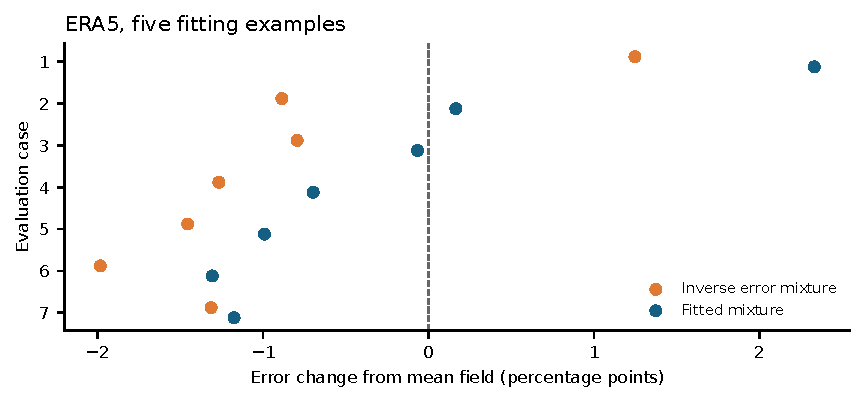
\includegraphics[width=.82\linewidth]{figures/era5_case_errors.pdf}
\caption{\textbf{ERA5 gains by evaluation case.} Change from the training mean
in relative $L^2$ percentage points, averaged over three $K=5$ fitting
selections. Negative values favor the mixture. Case numbers identify archive
rows rather than dates.}
\label{fig:era5cases}
\end{figure}

Predictions and losses use a $128\times256$ working grid, while the native
fine array has $721\times1440$ values. The input variables describe supplied
simulation drivers, not an established forecast origin. Absolute units,
calendar coordinates, and the target transformation remain unverified from
the source arrays. Relative temperature error changes under an additive unit
offset, and the unweighted grid metric is not an area weighted global metric.
These results concern the registered field emulation task, not global climate
skill or operational forecasting.

\subsection{Additional evaluation inputs for Heat I}
\label{app:additionalheat}
This supplementary check uses the existing Heat I library on 40 new fitting
pool cases and 128 new evaluation cases. Three fitting selections share those
evaluation inputs. Table~\ref{tab:fresh} reports the three main rules
separately from the 22 dataset comparison. This single PDE check predates
the direct loss control in Appendix~\ref{app:geometry} and does not establish
generalization to new problem families.

\begin{table}[h!]
\centering\small
\caption{\textbf{Additional Heat I inputs.} Mean relative $L^2$ errors in percent.
Three fitting selections share the same 128 evaluation inputs and trained models.}
\label{tab:fresh}\begin{tabular}{rrrrr}
\toprule
$K$ & \shortstack[r]{Selected\\model} & \shortstack[r]{Inverse\\error\\mixture} & \shortstack[r]{Fitted\\mixture} & All pairs FNO \\
\midrule
5 & 0.008638 & 0.005300 & 0.005454 & 0.011171 \\
10 & 0.008638 & 0.005286 & 0.005359 & 0.011171 \\
20 & 0.008638 & 0.005270 & 0.005296 & 0.011171 \\
\bottomrule
\end{tabular}

\end{table}

\clearpage
\section{Mathematical explanation and related systems}
\subsection{Error geometry and the fitting objective}
\label{app:geometry}
For a fixed library, Equation~\eqref{eq:riskmain} expresses expected squared
relative error as $R(w)=w^\top Cw$, with $C=\E[G(x,y)]$. The error product
matrix is uncentered, so shared bias remains part of the risk. Its diagonal
describes individual accuracy and its cross terms describe error alignment
\citep{breiman1996,krogh1994}. Writing $d_m=\widehat C_{mm}>0$, minimization
of the diagonal approximation $\sum_m d_mw_m^2$ under simplex constraints
gives $2d_mw_m=\lambda$. The scalar $\lambda$ enforces the unit sum constraint,
so normalization yields $w_m\propto d_m^{-1}$. This recovers the inverse error
mixture before its numerical floor, without assuming independent model errors.
If some $d_m=0$, an optimum is supported on the zero error entries.

For one case, let $e_m$ be model $m$'s normalized error field and
$r_m=\norm{e_m}_Q$ its magnitude. The improvement relative to errors of the
same sizes that all point in one direction is
\begin{equation}
 \left(\sum_m w_m r_m\right)^2-w^\top Gw
 =2\sum_{m<n}w_mw_n\left(r_mr_n-\langle e_m,e_n\rangle_Q\right)\geq0.
 \label{eq:direction}
\end{equation}
Here $G$ is the same case's error product matrix, and $m<n$ counts each model
pair once. Expansion gives the equality and Cauchy Schwarz gives nonnegativity.
The identity explains how errors in different locations or directions can help
either mixture. Negative correlation is not required, and the identity does
not establish that a small fitting set will discover useful weights.

The fitting criterion can change the preferred mixture \citep{acar2009,acar2015}.
Our joint fit minimizes mean squared relative error, whereas reporting uses
\begin{equation}
 L(w)=\E\!\left[\sqrt{w^\top G(x,y)w}\right].
 \label{eq:reportedrisk}
\end{equation}
Here $L$ averages the relative $L^2$ error over inputs and targets, taking
the square root separately for each field. Jensen's inequality gives
$L(w)\leq\sqrt{R(w)}$ for fixed weights, but does not equate their minimizers.
For example, two equally likely scalar cases with normalized model errors
$e_A=(0,2)$ and $e_B=(1.1,1.1)$ give
\begin{equation}
 L(t)=1.1-0.1t,\qquad R(t)=1.21-0.22t+1.01t^2,
\end{equation}
where $t\in[0,1]$ weights model A and $1-t$ weights B. The minimum of $L$
is at $t=1$, while $R$ is minimized at $t=11/101$, where $L=110/101$.
Thus fitting squared error can be about $8.9\%$ worse on the reported metric
even with unlimited fitting cases. Constant spatial fields give the same example.

\paragraph{Direct fitting of the reporting metric.}
A standard convex alternative fits the unsquared error directly:
\begin{equation}
 \min_{w\in\Delta_M}\frac1K\sum_{i=1}^K\sqrt{w^\top G_iw}
 =\min_{w\in\Delta_M}\frac1K\sum_{i=1}^K\norm{A_iw}_2,
 \qquad A_i^\top A_i=G_i.
 \label{eq:metricfit}
\end{equation}
Here $A_i$ factors the error matrix of fitting field $i$, $K$ counts fields,
and $\Delta_M$ contains nonnegative weights summing to one. Each term is a
norm of a linear map. Introducing upper bounds $t_i$ with
$\norm{A_iw}_2\leq t_i$ gives a second order cone problem. We evaluate this
loss control on 51 partitions of the original 17 PDE tasks at $K=5$, keeping
all predictions and case assignments fixed. The weights were saved before
their new scores were computed, but the predictions had previously been
inspected, making this a retrospective diagnostic separate from the three
main rules.

CVXPY 1.9.2 and Clarabel 0.11.1 solve the scaled problem with absolute and
relative gap tolerances $10^{-10}$ and feasibility tolerance $10^{-9}$.
All 51 solves returned optimal status. Eigenvalues below zero are clipped
only within $10^{-12}$ of spectral scale, with larger violations rejected.
The worst relative eigenvalue was approximately $-1.04\times10^{-18}$ and the
largest simplex residual before clipping and renormalization was
$4.15\times10^{-11}$. Source identities, reference error replay, and solver
records are retained with the locked fits.

\begin{table}[h!]
\centering\small
\caption{\textbf{Fitting the reporting metric directly.} Ratios compare with
the Selected model on the 17 PDE diagnostic tasks at five fitting examples.
Wins and losses require more than 1\% change after averaging three partitions.
The direct loss fit is a supplementary control, not a fourth main rule.}
\label{tab:losscontrol}\begin{tabular}{lrrrr}
\toprule
Method & Class ratio & Dataset ratio & Wins & Losses \\
\midrule
Inverse error mixture & 0.882 & 0.924 & 11 & 4 \\
Fitted mixture & 0.876 & 0.918 & 12 & 5 \\
Relative $L^2$ fit & 0.859 & 0.898 & 12 & 5 \\
\bottomrule
\end{tabular}

\end{table}

Direct relative $L^2$ fitting reduces class aggregated error by $2.0\%$ and
dataset aggregated error by $2.1\%$ relative to the original squared error
fit. Nine datasets improve by more than 1\%, none worsens by that margin,
and eight remain within 1\%. Against the Selected model, 12 improve and five
worsen. The result identifies a consequential loss choice without establishing
a new weighting principle or independent validation.

\subsection{What estimating the error matrix guarantees}
\label{app:proof}
\begin{proposition}[Error estimation and mixture risk]
\label{prop:bound}
If $\max_{m,n}|\widehat C_{mn}-C_{mn}|\leq\epsilon$ and a feasible
$\widehat w$ has empirical objective within $\delta\geq0$ of the simplex
minimum, then
\begin{equation}
 R(\widehat w)-R(w^*)\leq2\epsilon+\delta,
 \label{eq:bound}
\end{equation}
where $w^*$ minimizes population squared relative risk over the simplex.
\end{proposition}
Here $\epsilon$ bounds matrix estimation error and $\delta$ bounds numerical
optimization error. For every feasible $w$, nonnegative unit sum weights give
$|w^\top(\widehat C-C)w|\leq\epsilon\sum_{m,n}w_mw_n=\epsilon$.
Applying this once at $\widehat w$ and once at $w^*$, with empirical near
optimality between them, proves the result. The bound separates estimation
from optimization error but does not certify small $\epsilon$ from five
fields. Standard concentration arguments \citep{hoeffding1963} require
bounded error products and independent fitting fields, assumptions not
established here. Spatial pixels are not independent fitting examples.
The companion package retains the longer concentration calculation, whose
bound is weaker than a trivial bounded risk guarantee at the reported budgets.
Neither calculation establishes near optimality for the unsquared metric $L$.

\clearpage
\subsection{Relationship to the closest prior systems}
\label{app:prior}
Model weighting, automated surrogate selection, and multifidelity field
emulation are established ideas. Table~\ref{tab:prior} identifies these
precedents and the scope of our integration. The contribution is the adapted
portfolio, common parameter input interface, and experiments with counted
fitting examples. The table compares formulations rather than measured
performance. Direct comparisons with complete engineering automation systems
would require matched training, tuning, and information budgets.

\begin{table}[h!]
\centering\small\setlength{\tabcolsep}{3pt}
\caption{\textbf{Prior systems and the scope of this study.} These workflows
were not all evaluated on the present tasks. Adapted baseline implementations
do not substitute for complete system comparisons.}
\label{tab:prior}
\begin{tabular}{p{.24\linewidth}p{.31\linewidth}p{.36\linewidth}}
\toprule
Predecessor & Established contribution & Present investigation \\
\midrule
Engineering ensembles \citep{acar2009,viana2009} & Validation based weighting
and model selection. & Neural field library with several fidelity strategies
and counted fitting examples. \\
Functional output benchmark \citep{brunel2025} & Unified comparison of
multifidelity field emulators. & Heterogeneous neural and reduced basis
candidates combined from saved fields. \\
Stacking and AutoGluon \citep{wolpert1992,erickson2020} & Automated library
combination. & Whole field loss over a fixed portfolio of fidelity strategies. \\
EL MFS and AQBMF \citep{wang2024elmfs,lee2026aqbmf} & Adaptive LF fusion and
MF strategy selection. & Diverse field architectures with parameter only inference. \\
MAESTRO \citep{kim2026maestro} & LF and discrepancy families with screening
and leave one out selection. & Direct, correction, and fine only field models. \\
LANE SI \citep{borisova2024} & Neural and climatological spatial forecast
ensembles. & Parametric emulation with supplied multifidelity simulations. \\
HyperNOs \citep{ghiotto2025} & Automated operator training and hyperparameter
search. & Fitting weights across different fidelity use strategies. \\
MFRNP and MF DeepONet \citep{niu2024,howard2023} & Multifidelity field
architectures. & Common ensemble fitting over multiple adapted families. \\
\bottomrule
\end{tabular}
\end{table}

\clearpage

\section{Reproducibility, AI use, and ethics statements}
\label{app:statements}
\subsection{Reproducibility statement}
We will release the benchmark datasets and the code used to train and evaluate
all baseline implementations, the nine surrogate models, and the ensemble methods,
together with data preparation scripts, fixed splits, experiment configurations,
and scripts for reproducing the reported tables and figures.

We retain the datasets, training and simulation code, data preparation routines,
and experiment records for all 22 datasets in the benchmark and experiment
archives. The manuscript package supplies numerical snapshots, plotting and
table scripts, a workbook, and a portable program for fitting ensembles from
saved predictions and combining new predictions without their evaluation
answers. Input identities, source hashes, saved weights, and replay checks
connect these artifacts to the reported scores. The verified clean rebuild
covers ensemble fitting, saved prediction evaluation, tables, and figures.
It does not retrain the library or rerun the simulation solvers. The companion
supplement indexes enlarged dataset panels, exploratory experiments, and
detailed audit records omitted from the condensed appendix.

\subsection{AI use statement}
Generative AI assisted hypothesis development, experiment design, coding,
provenance inspection, result interpretation, mathematical analysis, literature
search, writing, visualization, and references. Reported values come from
experiment artifacts and are checked automatically. Scientific claims and
source attributions remain the authors' responsibility.

\subsection{Ethics statement}
Inaccurate field predictions can mislead engineering or climate decisions.
Benchmark error alone establishes neither physical validity nor operational
suitability. Dataset limitations and the scope of the ERA5 metric are disclosed
in the evaluation protocol and climate appendix. Data provenance and
redistribution permissions require review before public release.

\end{document}
